\documentclass[a4paper]{article}

\usepackage[utf8]{inputenc}
\usepackage{amsmath}
\usepackage{graphicx}
\usepackage{fancyhdr}
\usepackage{tabularx}
\usepackage{listingsutf8}
\usepackage{lmodern}  % for bold teletype font
\usepackage{amsmath}  % for \hookrightarrow
\usepackage{xcolor}   % for \textcolor
\lstset{
  columns=fullflexible,
  frame=single,
  breaklines=true,
  postbreak=\mbox{$\hookrightarrow$\space},
}
\usepackage{hyperref}
\usepackage{etoolbox}% http://ctan.org/pkg/etoolbox
\usepackage{needspace}% http://ctan.org/pkg/needspace
\usepackage{amsthm}

\usepackage[colorinlistoftodos,prependcaption,textsize=tiny]{todonotes}

%\Bearbeitet Format, sodass statt der Einrückung bei Paragraphen durch Zeilenabstand ersetzt wird
\usepackage{parskip}
\setlength\parindent{0pt}

%\Setzt Dokumentinformationen
\title{Master-Thesis: Incremental Analysis of Software Product Lines}
\author{Moritz Fl\"oter}
\date{June 2018}


\begin{document}
\bibliographystyle{unsrt}

\newtheoremstyle{mystyle}% name
  {3pt}%Space above
  {3pt}%Space below
  {\normalfont}%Body font
  {0pt}%Indent amount
  {\bfseries}% Theorem head font
  {}%Punctuation after theorem head
  {\newline}%Space after theorem head 2
  {}%Theorem head spec (can be left empty, meaning 'normal')

\theoremstyle{mystyle}


\newtheorem{req}{REQ}
\newtheorem{subreq}{REQ}[req]
\newtheorem{subsubreq}{REQ}[subreq]
\AtBeginEnvironment{req}{\Needspace{5\baselineskip}}
\setcounter{req}{0}

\newcommand*{\reqtable}[4]{
\begin{tabular}{ | p{0.15\textwidth} | p{0.79\textwidth} | }
	\hline
	\textit{Priority} & \begin{minipage}[l]{0.79\textwidth}
	\vspace{0.25em}
		#1
	\vspace{0.25em}
	\end{minipage} \\ \hline
	\textit{Source} & \begin{minipage}[l]{0.79\textwidth}
	\vspace{0.25em}
		#2
	\vspace{0.25em}
	\end{minipage}\\ \hline
	\textit{Description} & \begin{minipage}[l]{0.79\textwidth}
	\vspace{0.25em}
		#3
	\vspace{0.25em}
	\end{minipage} \\ \hline
	\textit{Explanation} & \begin{minipage}[l]{0.79\textwidth} 
	\vspace{0.25em}
		#4
	\vspace{0.25em}
	\end{minipage} \\
	\hline
\end{tabular}
}



%\Deckblatt
\maketitle
\newblock

\begin{center}
floeter@uni-hildesheim.de \par
Matrikel-Nr: 236278 \par
Supervisor: \par
Prof. Dr. Klaus Schmid \par
Christian K\"oher
\end{center}

\newpage
\lhead{{}}
\rhead{\leftmark}
\pagestyle{fancy}

\listoftodos[Notes]
\clearpage

%\Inhaltsverzeichnis
\tableofcontents
\newpage
\bibliographystyle{unsrt}

%\Deckblatt
\maketitle
\newpage

\setcounter{page}{1}
\lhead{{}}
\rhead{\leftmark}
\pagestyle{fancy}



\section{Introduction}


\todo{Nicht vergessen: Aufbau der Arbeit erneut beschreiben}

\clearpage
\section{Background}

In this section, the reader will be provided with a general introduction to Software Product Lines and the Linux kernel Product Line specifically. This builds the foundation for understanding analyses on Software Product Line that are introduced subsequently. Before diving into the concepts of incremental analyses in the following chapters, the software project KernelHaven is introduced as an infrastructure for performing analyses on Software Product Lines. KernelHaven itself will be used as the foundation for the practical implementation of our approach.

\subsection{Software Product Lines}\label{spl}

When starting a new software project from scratch, one approach is to write code specifically for that project. The codebase and the documentation are tailored to the needs and requirements currently at hand. And when another project is to be implemented, you do the same thing there. However it might turn out that those two projects technically share common functionality eventhough each product has features that the other does not.

Instead of writing code for one project specifically it might have made sense to create something that is configurable to cover multiple use-cases across different projects. Then for the next project it would be possible to combine and configure existing developed artifacts. And after some more projects it is perhaps even possible to realize a new product just by configuring and combining the assets that have already been created. This is where Software Product Lines come in. In contrast to traditional software development, Software Product Lines aim to reuse existing assets instead of writing software from scratch.

Software Product Lines use engineering techniques for creating a portfolio of similar systems from a shared set of software assets \cite{intro-spl}. This differenciates Software Product Lines from software systems with \emph{opportunistic} reuse. \emph{Oppurtunistic} reuse of single components occurs in many software projects where parts of an developed system are reused by other components or included as library within other projects. However Software Product Lines are actively built for reuse, thereby employing a \emph{predictive} reuse system, that directly aims for future products to be able to reuse created assets.

While considering configurability and reusability of assets when developing a single product results in a higher initial effort, the break even point is usually reached after about three products. Therefore incorporating the principles of Software Product Lines is advantageous when multiple system are able to share the same assets. Through the reuse of existing assets across multiple products, the development, maintainance and documentation effort is drastically reduced. Furthermore a new product is most likely more reliable and secure as it can be built directly on top of mature components  \cite[p.4f]{spl-in-action}.

There are three types of characteristics within Software Product Lines, that can be differenciated \cite[p.8]{spl-in-action}:
\begin{description}
\item[Commonality]  A characteristic that is shared across all members of the product line.
\item[Variability]  A characteristc that is included in some, but not all members of the product line.
\item[Product-specific]  A characteristic that is only included within one product. 
\end{description}

We consider characteristic of a Software Product Line to be a feature. Features within a software product line can be visualized using a feature model diagram as shown in \autoref{featuremodel}. 

\begin{figure}[h] 
  \centering
  \begin{minipage}[b]{1\textwidth} 
    \caption[Feature Model]{Feature Model for an Operating System}\label{featuremodel}
    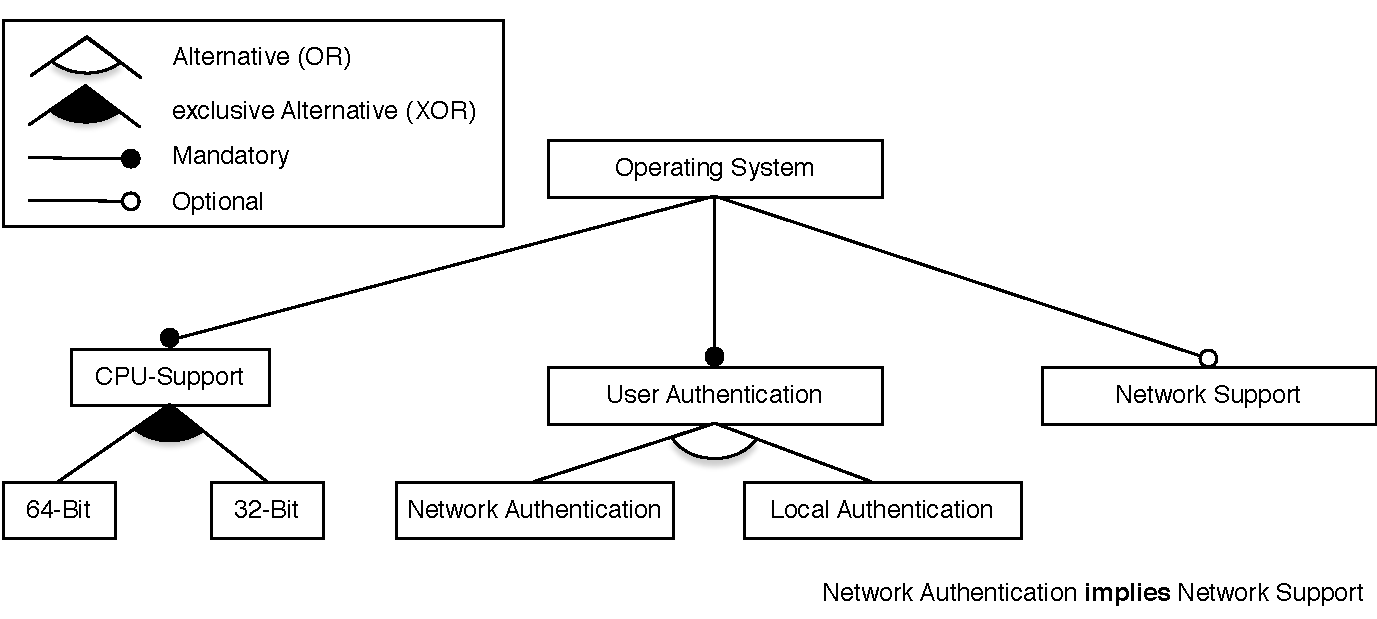
\includegraphics[width=1\textwidth]{img/featuremodel.pdf}
  \end{minipage}
\end{figure}

In the example, the operating system has to include support for a CPU through either a 32-Bit or 64-Bit option. While CPU-Support itself is a mandatory feature, the choice between the 32-Bit and 64-Bit option is an exclusive one. When choosing one option, the other option can not be included. The selection of both Network Authentication and LocalAuthentication is however possible for the User Authentication feature as the choice between them is not exclusive. However Network Authentication requires the selection of Network Support which would otherwise be an optional feature. The feature model is one example of how variability within a Software Product Line can be represented. Another textual representation of variability will be introduced in section \ref{linux-kernel} in the context of the Linux kernel Product Line. 

Those variability models represent configuration options and their dependencies within a Software Product Line. However the variability model does not represent how configured options are translated into the final product. In order to cover this process as well, we use two other models, the build and the code model. The consideration of three components related to handling variability within a product line can also be found in previous work \cite{nadi-linux-kernel} \cite{mining-kbuild} \cite{KroeherEl-SharkawySchmid18}.

The build model represents how the build systems how a concrete configuration is realized when building a product. A build system automates the process of program compilation. Its primary task is to create executables. For the build system of Software Product Line this means that it can carry the responsibility for selecting or even modifying compilation targets according to a concrete configuration. Following our example, the source-files related to the Network Support feature only need to be included into the build when the feature has been selected. The generic elements for the CPU-Support Feature on the other hand must be included at all times as they are a commonality for the product line. 

As the selective compilation of sourcecode is a mechanic that works before or at compilation time, it represents the implementation of compile-time variability. This is however not the the only option for achieving variability within a product. Another option is to modify the product is started (load-time variability) or executed (run-time variability) \cite[p.49]{Apel:2013:FSP:2541773}. It is for example possible to include more than one user interface for the same product and allow the user to select his preference even after the system has been compiled. While all three approaches allow the configuration of features within a within a software project, they differ in the binding-time of the feature. 

Finally different behaviours for different configured options may also be defined through the sourcecode. This can be achieved by using conditional compilation. In conditional compilation, compiler directives are used to include or exclude code sections from compilation. Those directives allow it to incorporate the selection or deselection of a certain feature for the selection or deselection of code sections. Not all programming languages use specific directives: In Java, the compiler recognizes if statements that always evaluate to false and ignores the encapsuled code for compilation. Compiler directives as interpreted by the C-Preprocessor do however share a strong resemblance to the if statements known from java or other programming languages. Those \texttt{\#ifdef} blocks check whether a certain parameters have been defined and evaluate conditions defined for the \texttt{\#ifdef} block to either include or exclude code from compilation. If the parameters are defined according to a concrete configuration based on the variability of a Software Product Line, they can be used to reflect configuration choices.

In this section, we covered Sofware Product Lines and gave an idea of how variability within a software project can be achieved. In the following section, we will take a closer look at how variability is incorporated in the Linux Kernel project.

\subsection{The Linux Kernel}\label{linux-kernel}

A prominent example for a Software Product Line in the operating system domain is the Linux Kernel. The Linux Kernel handles variability utilizing the conditional compilation of the C-Preproecessor as a core component. When implementing incremental analyses, we will rely on KernelHaven \cite{KroeherEl-SharkawySchmid18} as an existing software project that is able to work with C-preprocessor Software Product Lines that is introduced in section \ref{kernelhaven}. Eventhough other C-preprocessor Software Product Lines exist, many of them stem from a commercial context and are closed-source while the Linux Kernel is an open-source project. In order to enable the reproduction of our results as well as accessibility to the components used for this work, the Linux Kernel was chosen as target for evaluating the developed incremental analysis. The Linux kernel itself comes with more than 10.000 configurable features \cite{Tartler:2011:FCC:1966445.1966451}. 


\autoref{linux-build} shows an overview over the Linux Kernel build process. The Linux build system relies on KConfig files, Kbuild makefiles and code files to implement variability within the Linux Kernel Product Line. The files are processed by three components, the Kconfig-System, the Kbuild-System and finally the compiler. Kconfig defines configurable options and their dependencies while the Kbuild system is the build system used to automate the compilation process. The gcc compiler finally compiles codefiles to a linux variant that can be distributed and executed.

\begin{figure}[h] 
  \centering
  \begin{minipage}[b]{1\textwidth} 
    \caption[Linux build process]{Linux Kernel Build Process \cite{nadi-linux-kernel}}\label{linux-build}
    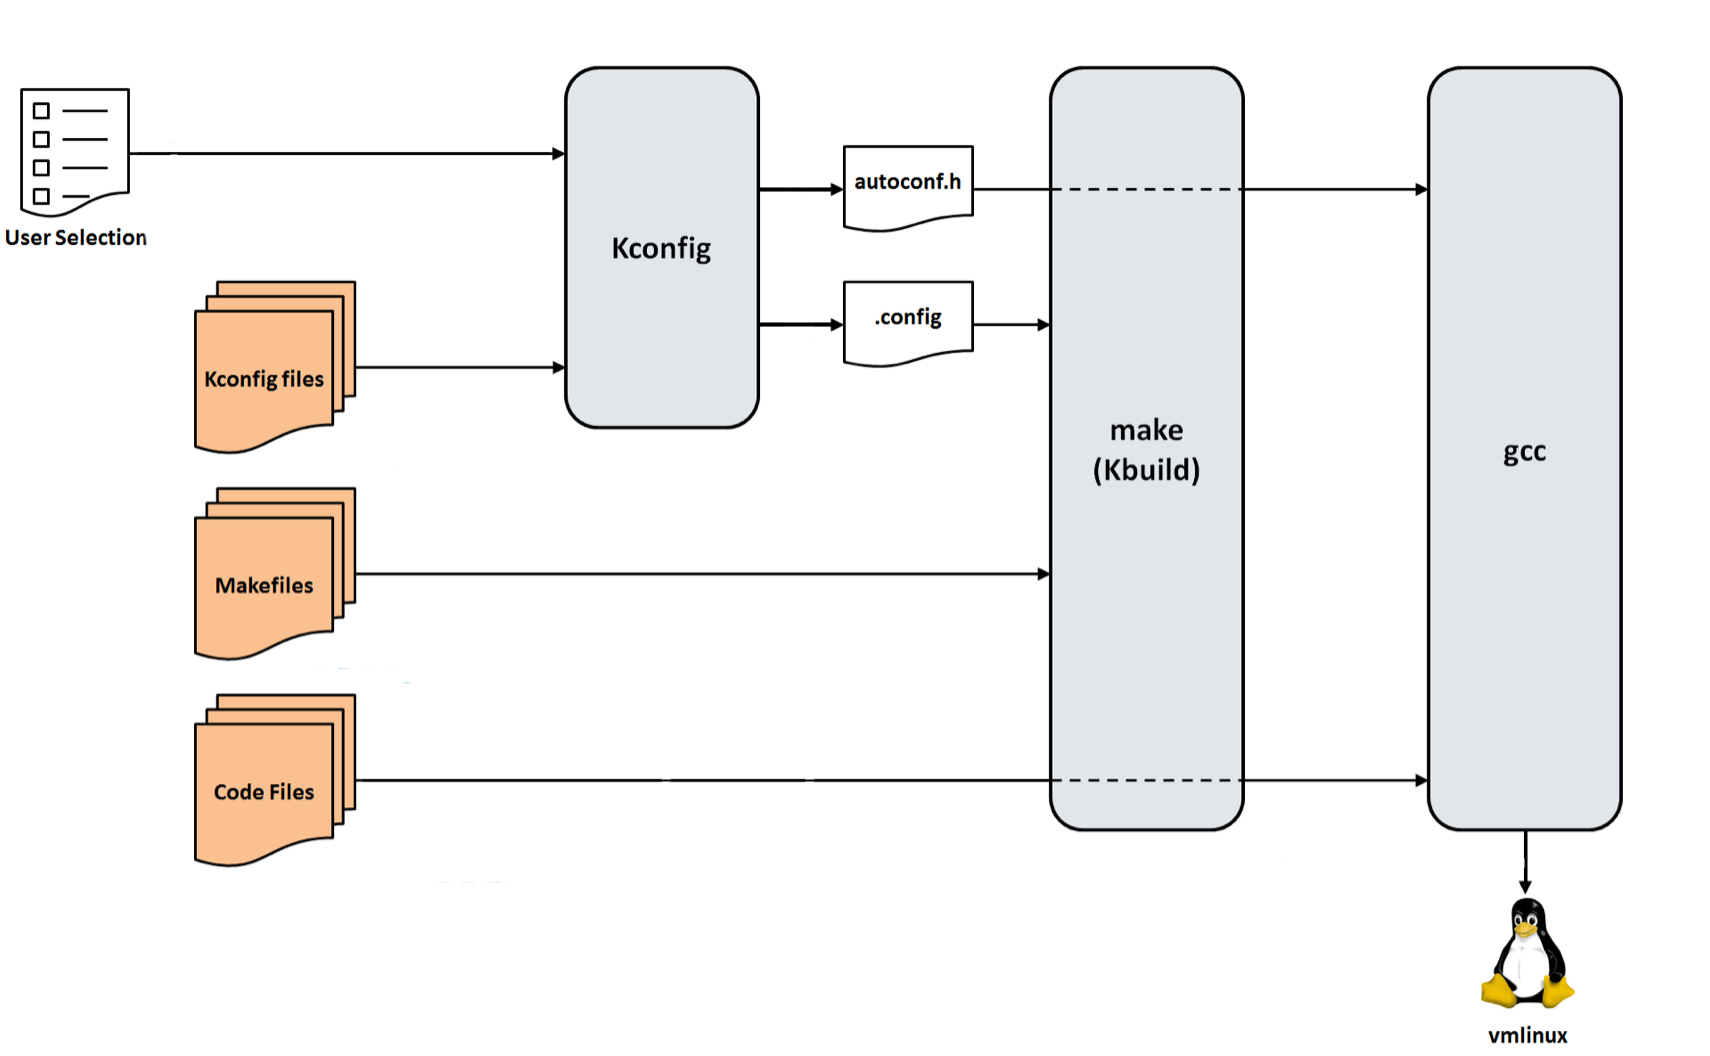
\includegraphics[width=1\textwidth]{img/linux-build.png}
  \end{minipage}
\end{figure}


Linux uses a the KConfig language to specify available configuration options and dependencies among them \cite{variabilitymodel-linux}. Thereby the KConfig files define the variability model of the Linux Kernel. 

\begin{lstlisting}[caption= KConfig Language, label=kconfig]{language=KConfig}
config NETWORK_AUTHENTICATION
	bool "Network Authentication"
	depends on USER_AUTHENTICATION
	select NETWORK_SUPPORT
	select REMOTE_USER_FOLDER_SUPPORT if NETWORK_STORAGE_SUPPORT
	default y
	help
	  Support for network authentication ...
\end{lstlisting}
 
Building on top of the example shown in \autoref{featuremodel} in subsection \ref{spl}, \autoref{kconfig} shows how KConfig can be used to describe the variabilitymodel. The example uses a boolean variable that allows for either inclusion or exclusion of a feature in the configured product. However Kconfig also offers an alternative option for including or excluding a feature: Tristate variables allow a feature to either be excluded, linked into the kernel statically, or be dynamically loadable \cite{variabilitymodel-linux}. Therfore the KConfig language allows the definition of the binding time for a certain feature. Other types of variables used in the KConfig language are integer and string.

In the example, NETWORK\_AUTHENTICATION can only be selected if USER\_AUTHENTICATION has also been selected as NETWORK\_AUTHENTICATION depends on this feature. If NETWORK\_AUTHENTICATION is selected for inclusion in the compiled product, the features prefaced with \texttt{select} are automatically included aswell. It is also possible to define more complex condition for \texttt{select} or \texttt{depends on} entries where the selection of a feature depends on more than one feature. In this instance REMOTE\_USER\_FOLDER\_SUPPORT is automatically selected if the NETWORK\_STORAGE\_SUPPORT feature is also configured to be included. Finally, help defines a text to provide the configuring user with information about the feature. This text is used in user interfaces for configuring the linux kernel such as menuconfig or xconfig.

The output of the configuration is a \texttt{.config}-file representing a concrete configuration aswell as a header file called \texttt{autoconf.h}. The Kbuild build system uses the generated configuration together with Kbuild makefiles to define which sourcefiles to include for compilation. Because the Kbuild makefiles define the build process of the product line, they represent the build model. Kbuild works by recursively processing the Makefiles within the directories and subdirectories of the Linux Kernel project to create two distinct lists containing objects that are to be included for the compilation process. The list obj-y contains all files that are to be compiled and linked whereas  obj-m contains those that will be compiled as loadable modules \cite{nadi-linux-kernel}\cite{makefiles.txt}. 

Finally \texttt{autoconf.h} defines variables for each selected KConfig feature \cite{Tartler:2011:FCC:1966445.1966451}. Defined variables within \texttt{autoconf.h} are used to evaluate compiler directives for including or excluding code sequences. \autoref{conditional-compilation} shows an examplary excerpt of source code. Lets assume that \texttt{autoconf.h} contained the line \texttt{\#define CONFIG\_NETWORK\_SUPPORT}. Because \texttt{CONFIG\_NETWORK\_SUPPORT} is defined and set to \texttt{1}, the \texttt{\#ifdef} statement in our example evaluates to true and therefore the line \texttt{include <network/generic\_driver.h>} is included for compilation of the  linux variant.

\begin{lstlisting}[caption=Conditional Compilation within the Linux Kernel, label=conditional-compilation]{language=C}
 # ifdef CONFIG_NETWORK_SUPPORT
 #  include <network/generic_driver.h>
 # endif
\end{lstlisting}

The code, build and variability model as described through the files within the Linux Kernel project can be used to perform analyses on the Sofware Product Line wich are introduced in the next section.

\newpage

\subsection{Software Product Line Analyses}

Measuring of relevant parameters (e.g. performance), testing and analyzing products is well established for individual products \cite[p.243]{Apel:2013:FSP:2541773}. 
In order to apply those methods on a the product line, a simple approach would be to analyze every possible permutation of feature combinations that is possible as a single product. For a product line with 33 independently selectable features and an analysis time of one second per permutation this would however result in an insurmountable computational effort of more than 272 years \cite{Thum:2014:CSA:2620784.2580950}. In section \ref{linux-kernel}, we mentioned that the Linux Kernel has more than 10.000 configurable features. Therefore approaches that exist for individual products do not scale for product lines. Furthermore aspects of variability itself within a software project can also be used as working base of analyses thereby adding a dimension to the analysis of individual products.

This section will provide an overview of analyses that are tailored towareds Software Product Lines. As the KernelHaven which will be used for our implementation of an incremental analysis currently provides an infrstructure for static analyses, static analyses will be the focus of this section.

\subsubsection{Analysis Strategies}

Following previous work from Tartler et al. \cite{Tartler:2011:FCC:1966445.1966451}, we distinguish five different categories of analysis strategies:

\begin{enumerate}
	\item Product-based
	\item Family-based
	\item Feature-product-based
	\item Feture-family-based
	\item Family-proudct-based
\end{enumerate}


\todo{describe that feature-based or feature-family product based did not occur}



Thum et al. \cite{Thum:2014:CSA:2620784.2580950} propose a categorization


\todo{describe Software Product Line Analyses}

\newpage
\subsection{KernelHaven - An Analysis Infrastructure}\label{kernelhaven}

KernelHaven is a an infrastructure for variability-based analyses of C-preprocessor Software Product Lines such as the Linux kernel \cite{KroeherEl-SharkawySchmid18}. This section  provides an overview over the overall concept and features of KernelHaven and then describes the possibilites of extending KernelHaven through plugins. KernelHaven and its plugin infrastructure constitute the foundation for the system developed for incremental analyses that is described in section \ref{implementation}. 

Before diving into technical details, the some of the terminology used for the remainder of this work needs some clarification. The set of all files  that represent a software system and are used as input for an analysis will be referred to as the codebase. The codebase therefore includes files containing source code as well as files defining the build process or configuration-options. Referring to the Linux-Kernel as an example this would mean all files within the Linux repository for single revision of the kernel.
The term sourcefile or codefile on the other hand refers to a file that contains source-code. For the Linux kernel this would mean all *.c and *.h files. Finally variability model files and build model files are files within the codebase that relate to the respective models. For Linux this means that the files of the KBuild-system are considered variability model files, while files of the KConfig system are considered to be variability model files.

An overview over the KernelHaven-Architecture structure is shown in \autoref{pipeline}. Because KernelHaven targets C-preprocessor Software Product Lines, it needs to be able to process build-, variability and codemodel. KernelHaven achieves this by using extractors that extract data models from a given codebase. The analysis itself is then executed based on the extracted models. Extractors and analyses are configured as a pipeline through the PipelineConfigurator which uses a configuration-file to define the settings for the execution of KernelHaven. This configuration-file is translated into a configuration-object that then gets passed to each component of the pipeline by the PipelineConfigurator. It is  important to note that KernelHaven-plugins do not read their settings directly from a configuration file. This is because KernelHaven offers entry points to perform adjustments to the configuration described by the file through the configuration-object before it is used in subsequent steps.

\begin{figure}[h] 
  \centering
  \begin{minipage}[b]{1\textwidth} 
    \caption[KernelHaven-Pipeline]{KernelHaven-Architecture \cite{KroeherEl-SharkawySchmid18}}\label{pipeline}
    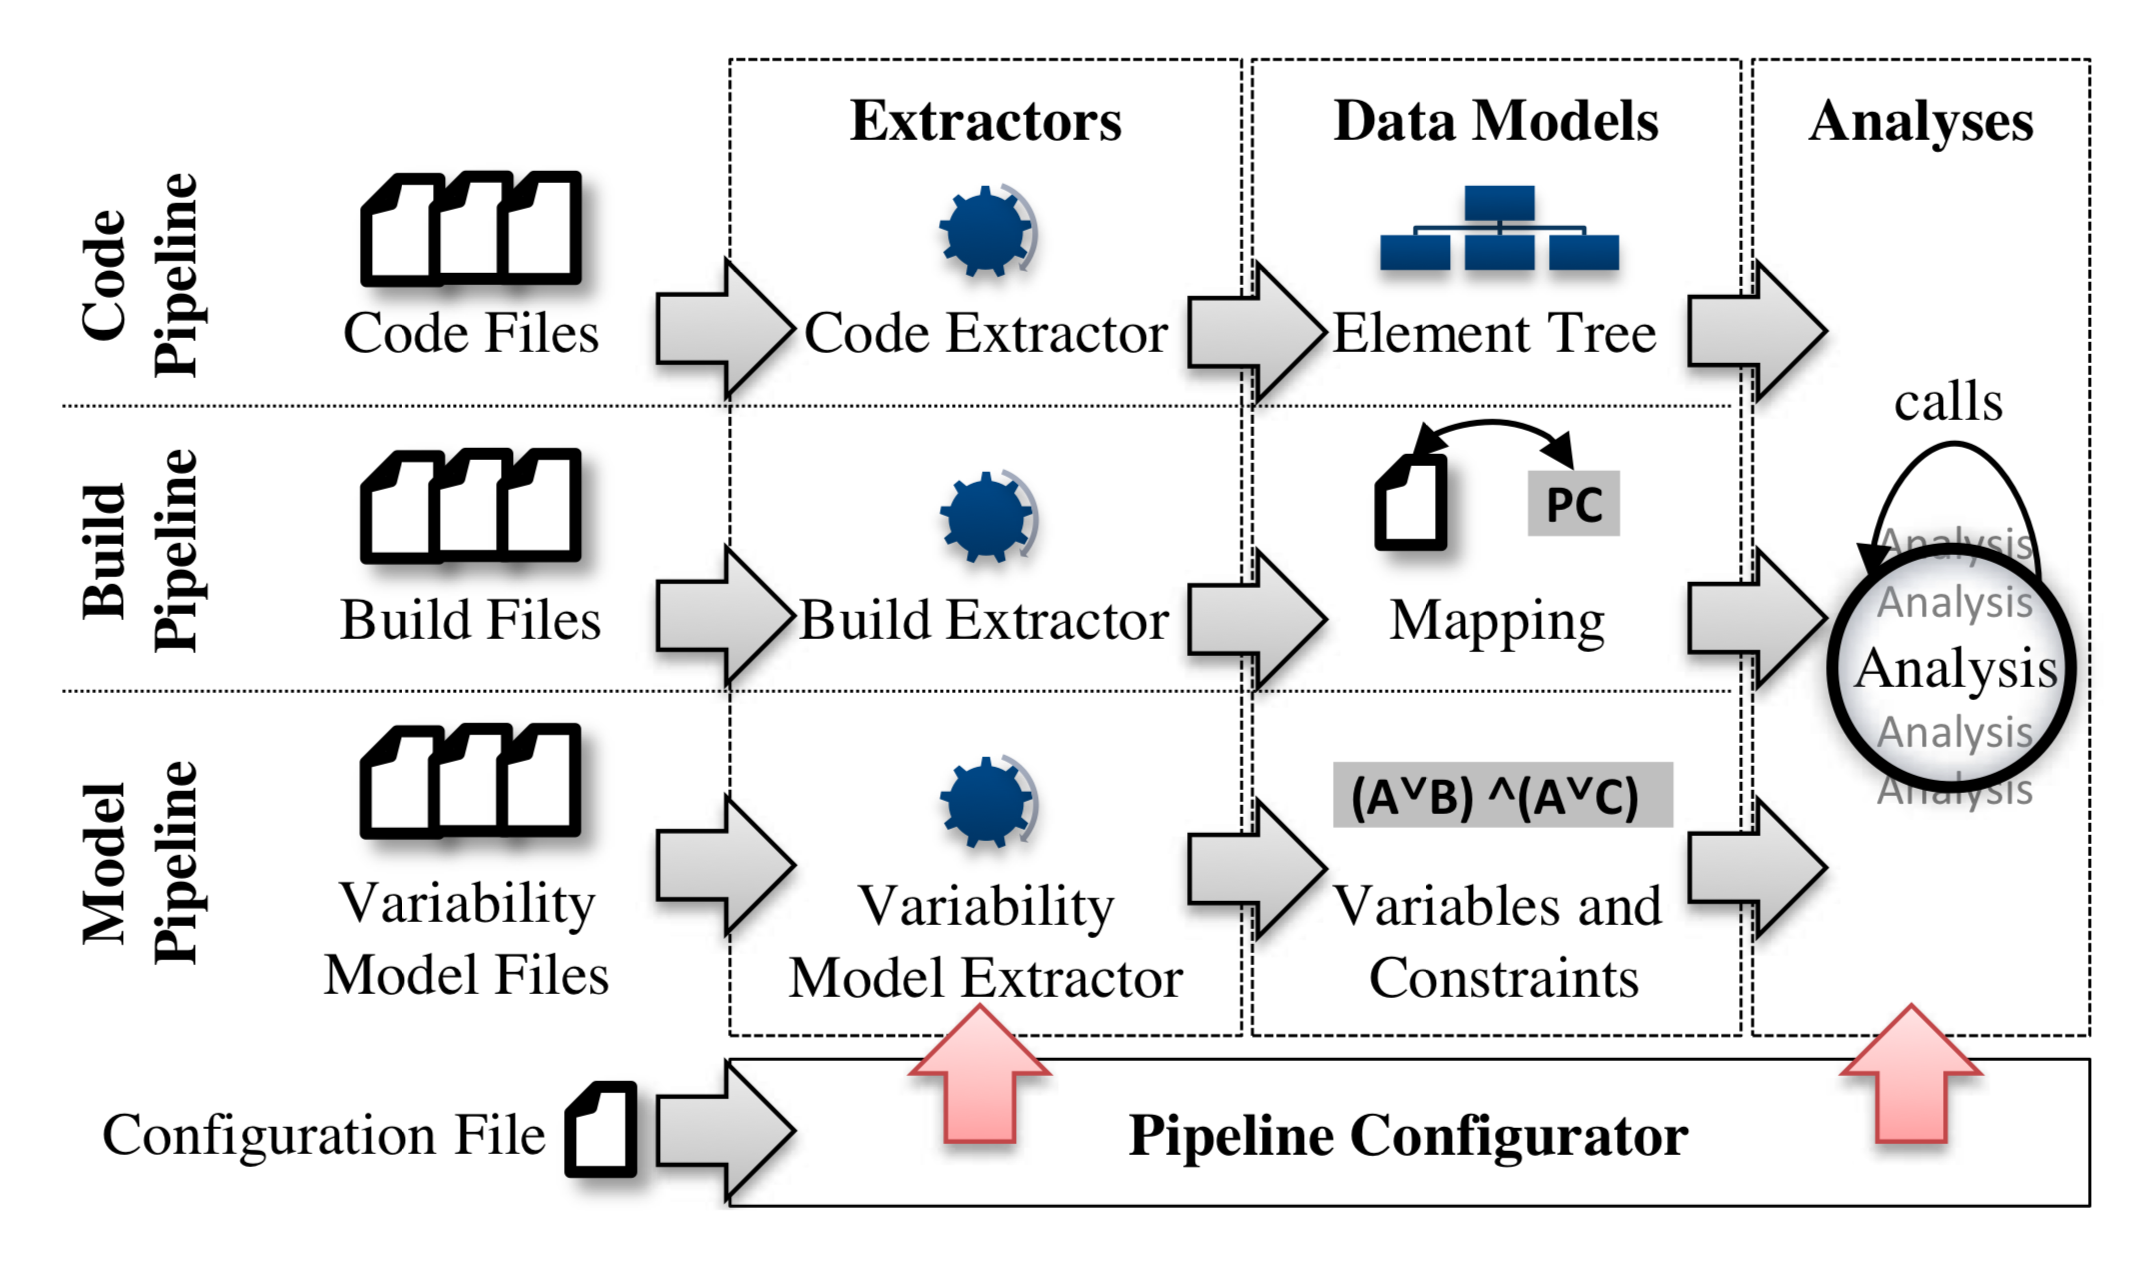
\includegraphics[width=1\textwidth]{img/KernelHaven-Pipeline.png}
  \end{minipage}
\end{figure}

By using a custom configuration-file, the user is able to configure existing Extractors and Analyses to suit his needs. However KernelHaven is also meant to be easily extendeable for developers and and therefore provides the possibility to extend the infrastructure through plugins.

KernelHaven can be extended through three types of plugins:

\begin{enumerate}
    \item Preparation-Plugins
	\item Extractor-Plugins
	\item Analysis-Plugins
\end{enumerate}

All of the plugins do not require adjustments to the main KernelHaven infrastructure but instead can be loaded as jar-files and automatically get added to the classpath when KernelHaven is started.

A preparation-plugin can define tasks that get executed before the KernelHaven-Pipeline is started. This can for example be useful for preprocessing inputs. Furthermore a PreparationPlugins allows to apply modifications to the configuration-object before the object is used by Extractor or Analysis-Plugins. However if no tasks need to be performed prior to the execution of the pipeline, no Preparation-Plugin needs to be defined for execution. 

Extractor-Plugins on the other hand are required to generate the models that the analysis can run on. There are three types of extractors: code-model extractors, variability-model extractors and build-model extractors. Different extractors may work based on different files within the codebase. Furthermore the results of two different extractors for the same type of model may vary even if the same codebase was analyzed. This becomes clear when looking at two of the existing extractors for the code-model. The TypeChef-Extractor based on the TypeChef-tool \cite{Kenner:2010:TTT:1868688.1868693} extracts a complete abstract syntax tree and uses macro expansion during the extraction of models from *.c files. The UndertakerExtractor based on the Undertaker-tool \cite{Tartler:2011:FCC:1966445.1966451} generates a representation of structure of \texttt{\#ifdef}-blocks.

While the KernelHaven infrastructure benefits from a selection of various extractors for the code-model, only one extractor is available for the build- and another for the variabilitymodel \cite{KernelHave-wh}. The buildmodel can be extracted using the KconfigReaderExtractor based on the KConfigReader-tool \cite{ck-kconfig} while the codemodel can be extracted through the KBuildMinerExtractor using the KbuildMiner-tool \cite{ck-kbuild}.

Both the KbuildMinerExtractor and the KconfigReaderExtractor are only able to extract the complete model represented through the codebase. This is not the case for the codemodelextractors which may also be configured to only process a subset of the files within the codebase. This is because the codemodel-extractor is able to individually process each sourcefile. Through header-files, extractors like the TypeChefExtractor might also consider other files when parsing one sourcefile. Nevertheless an individual model for each sourcefile is generated. This is not the case for KBuild and KConfig-files as the KBuild and KConfig-System both process complex dependencies that are spread between multiple files. Therefore the build- and variablity-model are built viewing the information from all KConfig and KBuild-files in total and not by looking at one individual file at a time.

Extractors may be configured to write extracted models to a cache-directory in order to reuse them for subsequent extectutions of KernelHaven removing the need to extract them again. Therefore KernelHaven does not necessarily require extractors to run for each execution of KernelHaven if the models already have been extracted before.

Finally Analysis-Plugins define the analysis that uses the extracted models. In order to ease the implementation of Analysis-Plugins, the plugins themselves do not have to take care of where the models come from. An analysis simply defines which models it needs and the corresponding extractors get started accordingly. This lets an analysis-developer focus directly on the work with the models themselves. Initially KernelHaven Analysis-Plugins  were single components that always processed the models directly. While the option to implement such an Analysis-Plugin still exists, KernelHaven also offeres the possiblity to implement AnalysisComponents that can be reused and combined to run after each other. An analysis that consits of such components is called a PipelineAnalysis. A PipelineAnalysis allows the result of one AnalysisComponent to be processed by the next one.  However only one result may be passed on to the next AnalysisComponent and only the first AnalysisComponent has access to the models. In order to provide a simple means of rearranging and recombining analysis components, a custom domain specific language is implemented in KernelHaven allowing to define chains of AnalysisComponents from within the configuration-file itself. In case the desired combination of AnalysisComponents requires intermediate tasks and does allow to simply pass on the result of one component to the next, AnalysisComponents may also be combined through java-code. This further improves the possibility for reuse of AnalysisComponents even if it requires to write custom code.

The KernelHaven main projects start page on github offers an overview over existing plugins. Later in this work, we will rely on exsiting AnalysisComponents within the UndeadAnalyzer-Plugin to implement an incremental Dead Code Analysis.

Of course any new plugin-implementation may reuse AnalysisComponents from other plugins aswell. Furthermore utility-plugins exist that do not satify any plugin-interface of KernelHaven directly but offer functionality to other plugins to ease their implementation. The UndeadAnalyzer for example relies on the CnfUtils plugin to provide SAT-solving capabilities.

\newpage
\section{Concept for Incremental Analyses}\label{concept}

KernelHaven and other software tools such as Undertaker\cite{Tartler:2011:FCC:1966445.1966451} currently allow to analyze a given codebase in its entirety. When changes to the codebase are introduced, the entire codebase must be analyzed again resulting in costly computations. This is because the model-extraction has to be redone and the subsequent analysis has to redo the computation for the new models. Assuming that an analysis consists of model-extraction and subsequent computations based on the extracted models, we are presented with two options to reduce computational effort:

\begin{enumerate}
	\item Reduction of computational effort for the extractors \\
	\emph{Extraction does not need to happen on the entire codebase - only the parts that changed dictate what to extract}
	\item Reduction of computational effort for the analysis performed on the extracted models \\
	\emph{Models do not need to be processed again completely - only the parts that changed dictate what to process}
\end{enumerate}

We refer to an analysis that utilizes one or both of those measures to reduce the computational effort when changes are introduced as an incremental analysis.

The first option can be achieved by the filtering of input files so that only files that were affected by changes need to be extracted. The most trivial possibility to reduce effort is to define that where a file was left unmodified, no new extraction needs to happen. 
However a file change does not necessarily result in changed variability information - and as models are extracted to obtain variability information, files where that information did not change can also be excluded. Filtering files based on changed variability further reduces the computational effort for obtaining the models. This kind of filtering can be used when every file is handled isolated from other files within the extraction logic.

While the described approach certainly makes sense for some scenarios, it does not suffice for others. If a file changes, it might affect the models of another file aswell if dependencies exist between those two files. Depending on whether or not the extraction logic includes those dependencies when building a model for a single file, different models might be computed for the same file even if the file itself is unchanged. An example for this is the extraction logic of TypeChef \cite{Kenner:2010:TTT:1868688.1868693}. Typechef uses macro expansion to compute the models for each sourcefile and thereby includes information from other files. 

Therefore filtering for direct file changes or variability changes within a single file is not sufficient for every situation. Instead it might be necessary to also include files that have been affected by the change. In order to keep the concept for incremental analyses generic enough to cover those use cases, different filtering mechanism must be applicable. However the extraction of a partial model is only possible if the extraction logic itself allows that. The existing code-model-extractors for KernelHaven  are able to run on a subset of files thereby extracting a partial model.  As already mentioned in section \ref{kernelhaven}, this is not the case for build-model and variability-model extractors. Therefore as soon as one of the related files changes, the entire model needs to be extracted. While we initially excluded

At the end of the extraction process, the complete code-, build- and variabilitymodel can be provided by merging the extracted parts with the models representing the previous state of the codebase. This allows the analysis to have full access to the models eventhough the computational effort was reduced for the extraction itself.

Now the second option can be applied. Depending on the analysis that is performed, it is possible that only a part of the models must be processed because the analysis-results for the other parts were unaffected by the changes to the codebase. The Dead Code Analysis is an example for an analysis that is able to work based on a partial code-model. The implementation of the Dead Code Analysis is described in \autoref{incremental-dead-code-analysis}.


\clearpage
\section{Requirements for the Software System}

This section lists the requirements for the developed software system that enables incremental analyses. The developed system consists of an infrastructure for incremental analyses as well as an concrete implementation of an incremental dead code analysis for this infrastructure.

The information on each requirement broken down to four fields:

\begin{description}
    \item [Priority]
	This describes the priority of a requirement. The priority is given through the keywords Must, Should and May. The usage of the definitions takes RFC 2119 \cite{RFC-bum} as a guideline. Therefore \underline{Must} describes a requirement that has to be implemented. \underline{Should} indicates that the implemenentation of the requirement is strongly desired. Not fulfilling a Should requirement  does however still result in an acceptable overall system if the Must requirements are met. Finally \underline{May} indicates a truely optional requirement. Those requirements represent additions to the system that are considered useful but at the same time are not valued as high as Must or Should requiirements.
    \item [Source]
    The Source-field describes the origin of the requirement.
    \item [Description]
    this field provides a description of the requirement.
    \item [Explanation]
    Explanation provides further deatail on the requirement and may additionally provide reasoning as to why the requriement is included.
\end{description}

\begin{req}[Working Base of an Incremental Analysis]
	\reqtable
	{Must}  {Interview}
	{An incremental analysis must work based on the current state of a repository and a proposed change. }
	{The working base of each incremental analysis is the previous state before a commit/code change. The increment is represented by the change introduced.}
	
	\begin{subreq}[Input Format for an Incremental Analysis] \label{req:git-diff}
		\reqtable
		{Must}  {Interview}
		{The input must be a git-diff file. Furthermore a codebase upon which the changes described in the git-diff file can be applied is required.}
		{The main input for the analysis is a git-diff file. This diff represents a changeset that is to be analysed.}
	\end{subreq}
\end{req}

\begin{req}[Covered Analysis-Types]
	\reqtable
	{Must}  {Initial Description, Interview}
	{The developed system must support block-based analyses. }
	{}
	
\end{req}


\begin{req}[Filtering of Extractor Input] \label{req:early-filtering}
\reqtable
	{Must}  {Interview}
	{The set of files within the codebase upon which the extractors operate should be reduced before being passed to the extractors.}
	{Because extraction is costly, the filtering of artifacts must happen before the extractors are called.}
\end{req}

\begin{req}[Processing of Partial Models] \label{req:early-filtering}
\reqtable
	{Must}  {Interview}
	{It must be possible for Analysis-Plugins to process partial models in order to reduce the computational effort.}
	{In order to reduce the execution time of an analysis as described in section \ref{concept}, mechansims need to be implemented that allow it to process partial models.}
\end{req}


\clearpage
\begin{req}[Configuration of Filters for Input-Files] \label{req:optimization}
\reqtable
	{Must}  {Initial Description}
	{
	The implemented infrastructure must provide means to configure different filters for the input.
    }
	{Depending on the extractor in use and the way it processes input files, different options cover different use cases. Furthermore different filters may affect the overall performance of the software system.}

\begin{subreq}[Implementation of Filters for Input-Files]\label{req:mandatory-filters}
    \reqtable
	{Must}  {Interview, initial description}
	{
	The filters listed below must be implemented (see REQ \ref{req:optimization}):
	\begin{itemize}
		\item \texttt{off} \\
		no filtering 
	    \item \texttt{change only} \\
	    only work with files that were modified
	    \item \texttt{variability-change only} \\
	     only work with files where the variability information was changed
	\end{itemize}
    }
	{In order to evaluate different filter methods and their effect on performance, different categories of filtering are required. \texttt{off} represents the state where no filtering is done, while \texttt{change only} performs superficial filtering without regarding variability information directly. Finally \texttt{variability-change only} is the most sophisticated filtering option of the three as it requires an analysis of the filecontent of each artifact itself.}
\end{subreq}

\begin{subreq}[Implementation of Effect-Filters for Input-Files]
    \reqtable
	{May}  {Interview, initial description}
	{
	The filters listed below may be implemented:
	\begin{itemize}
		\item \texttt{change-effect} \\
		work with files that were modified and files that were indirectly affected by the change (eg. through includes)
	    \item \texttt{variability-effect}  \\
	    work with files where the variability information was changed and files that were indirectly affected by the variability change
	\end{itemize}
    }
	{When a file is modified, it may affect other files as well that were not changed directly. Depending on the extractors and analyses used it may be necessary to analyze those files as well.}
\end{subreq}

\end{req}

\begin{req}[Rollback must be possible] \label{req:rollback}
\reqtable
	{Must}  {Interview}
	{It must be possible to revert back to the previous state after execution of an incremental analysis.}
	{An Analysis may change the source-files used as input for the extractors along with other changes. Those changes reflect the changes introduced by the new increment that was used as input. If that increment however contains defects identified by the analysis the user might choose to revert the changes and propose an alternative change. This alternative change can only be analyzed if KernelHaven reverts to the original state before the initial change.}

\end{req}

\begin{req}[Incremental Dead Code Analysis] 
\reqtable
	{Must}  {Initial description}
	{An incremental dead code analysis must be implemented}
	{The dead code analyis serves as a practical example for block based analyses. It is used to demonstrate and evaluate the effectiveness of the incremental approach.}
	
	

	
	\begin{subreq}[Incremental Dead Code Analysis Result Format] \label{req:format}
    \reqtable
    {Must}  {Interview}
	{The result should be given in the same csv-format as implemented in the existing UnDeadAnalyzer\footnote{\url{https://github.com/KernelHaven/UnDeadAnalyzer}} plugin for Kernelhaven.}
	{Maintaining the same format as the non-incremental dead code analysis allows for comparability between incremental and non-incremental analyses. \\
	\emph{Note: eventhough the csv-format remains unchangend, the contents of incremental and non-incremental result-files might differ (see REQ \ref{req:coverage})}}
	\end{subreq}
	
	\begin{subreq}[Incremental Dead Code Analysis Result Coverage] \label{req:coverage}
    \reqtable
    {Must}  {Interview, feedback from presentation of initial concept}
	{The analyis result should only contain elements that are results of the the latest analysis}
	{As the analysis should provide feedback for the developer on his work, parts of the software system which could not have been affected by the changes he introduced do not need to be represented in the result. Therefore merging the result of the increment with previous results is not desired.}
	\end{subreq}
\end{req}

\clearpage
\begin{req}[Target Artifacts] 
\reqtable
    {Must}  {Initial Description}
	{The software system must support the processing of *.c, *.h, makefile, Kbuild and Kconfig files}
	{The filetypes listed above represent the CodeModel, BuildModel and VariabilityModel of the Linux kernel. As the Linux kernel is used for the evaluation of the implemented incremental analysis approach, those filetypes need to be considered.}
\end{req}


\begin{req}[Run existing KernelHaven-Analyses incrementally] 
\reqtable
    {Should}  {Interview \\ \emph{Note: This requirement emerged after the implementation choice to use the KernelHaven infrastructure was made}}
	{It should be possible to run existing analyses incrementally without reimplementation.}
	{Existing analysis plugins for KernelHaven have been written as non-incremental analyses. The adaptation of existing analyses removes the need to reimplement existing analyses. Furthermore the adaptation of existing plugins allows for performance evaluation of incremental analyses against non-incremental analyses.}
\end{req}

\newpage

\section{Implementation of Incremental Analyses}\label{implementation}

This section describes the implemented infrastructure for incremental analyses and provides reasoning for the decisions made when engineering the infrastructure. The term 'incremental analyses' will henceforth be used as shorthand for  'block based incremental analyses' as other types of analyses are not targeteted by the infrastructure.

The infrastructure itself is based on KernelHaven\cite{KernelHaven} as KernelHaven together with its plugins provides a working implementation for various software product line analyses. Through KernelHaven's plugin interfaces, it is also possible to implement the infrastructure for incremental analyses as a plugin itself.

By extending an existing infrastructure like KernelHaven, we can benefit from an existing codebase as well as future developments within the KernelHaven project. Furthermore future users of the incremental infrastructure can adjust existing non-incremental analyses written for KernelHaven to run as incremental analyses.

\subsection{Two Phases of Non-Incremental Analyses}\label{2-phases}

The execution of an analysis in KernelHaven in most cases can be broken down to two mandatory phases: the Extraction-Phase and the Analysis-Phase. In the extraction phase, KernelHaven extracts models from the codebase  (or alternatively reads them from the cache). In the Analysis-Phase the resulting models are used to compute the analysis results. A simplified view of those phases is presented in \autoref{2-phases-image}.

\begin{figure}[h] 
  \centering
  \begin{minipage}[b]{1\textwidth} 
    \caption[Non-Incremental Analysis: Two Phases]{Non-Incremental Analysis: Two Phases}\label{2-phases-image}
    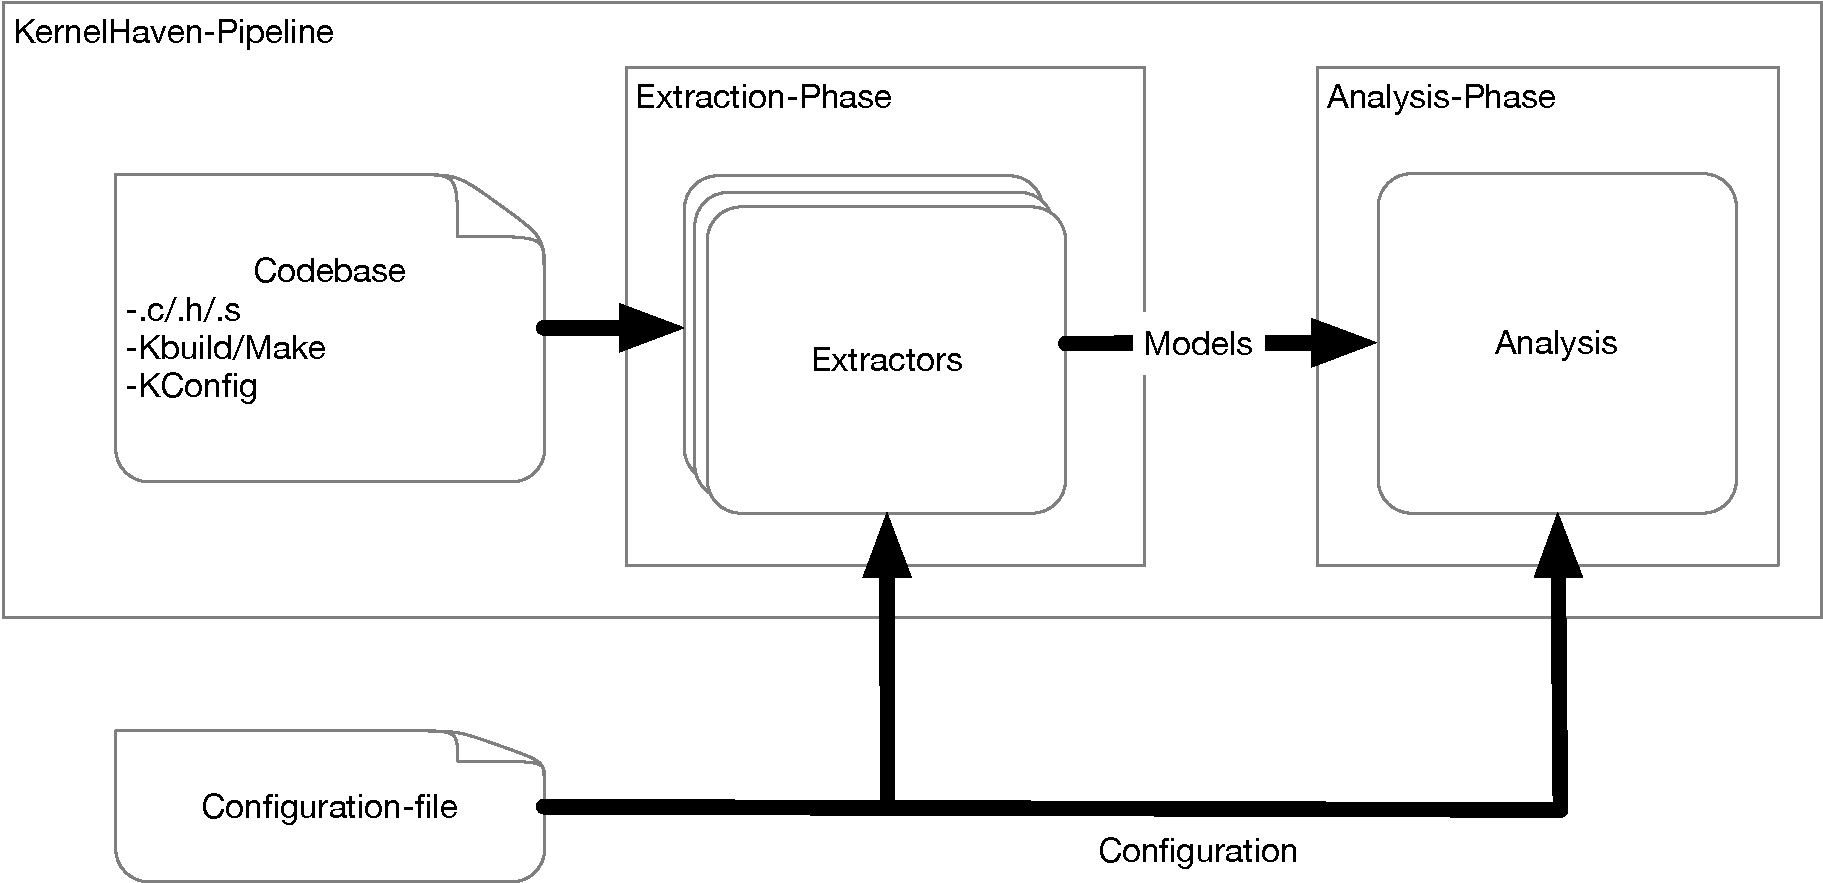
\includegraphics[width=1\textwidth]{img/KernelHaven.pdf}
  \end{minipage}
\end{figure}


While this view does ignore some technical aspects, it focuses on the core aspects of an analysis execution. Therefore it also does not try to replicate the configuration mechanism of KernelHaven and instead only visualizes the configuration of the pipeline components as a direct result of the configuration file. This simplification makes it easier to understand the required modifications for performing incremental analyses. Those modifications will be presented in the next section.

\subsection{Four Phases of an Incremental Analysis}

While the Analysis- and Extraction-Phase as described in \autoref{2-phases} are also present for analyses implemented with the incremental infrastructure, there are additional mandatory tasks which get executed in two more phases - the Preparation-Phase and the Post-Extraction-Phase. The resulting four phases are visualized in \autoref{4-phases}.

The Preparation-Phase is the first phase in an incremental analysis. Its purpose is to update the codebase and reduce the number of files that the extraction has to run on (see REQ \ref{req:early-filtering}). This saves computational effort when running the extractors as some parts of the codebase  may not need to be processed again. Instead the result of previous extractions may be reused. KernelHaven allows the configuration-object to define which files extractors run on. Therefore the configuration is not simply read from the configuration-file and passed on without modification but instead gets modified to only define a subset of the original files. This modification happens in the Preparation-Phase before the Extraction-Phase starts.

 But even before any filtering on the artifacts in the codebase happens, the incremental infrastructure ensures that the codebase represents the increment that is to be analyzed. This is possible to achieve by using a git-diff file describing changes to the codebase (see REQ \ref{req:git-diff}). In order to allow for reuse of existing extractors, the changes need to be applied to the codebase on the filesystem as the extractor-plugins for KernelHaven work based on access to the filesystem and can not work with data streams.

Because of the filtering performed in the Preparation-Phase, the analysis may not simply run on the result of the extractors directly as those would only generate a subset of the models. Therefore the result is merged with the results of previous extractions. After merging, it makes the resulting code-, build- and variabilitymodel available to the analysis through the \texttt{HybridCache}.

While merging the extractors outputs, it is important that no prior extraction results get overwritten. This is because REQ \ref{req:rollback} requires that the state before the execution of an incremental analysis can be restored. Therefore the Post-Extraction-Phase uses a modified implementation of the cache-system, that the main infrastructure of KernelHaven uses. This \texttt{HybridCache} allows storage and access to two versions of the code-, build- and variabilitymodel. It guarantees that the previous code-, build- and variabilitymodel can be restored.

While a rollback to previous extraction-results is the main reason for introducing the \texttt{HybridCache}, a side benefit is that analyses now may use both the current and the previous state of the codebase. This could be relevant for future implementations of incremental analyses that draw benefits from comparing the old and the new model. \todo{eventually discuss this in more detail? or reference to a later chapter}.

\begin{figure}[h] 
  \centering
  \begin{minipage}[b]{1\textwidth} 
    \caption[Incremental Analysis: Four Phases]{Incremental Analysis: Four Phases}\label{4-phases}
    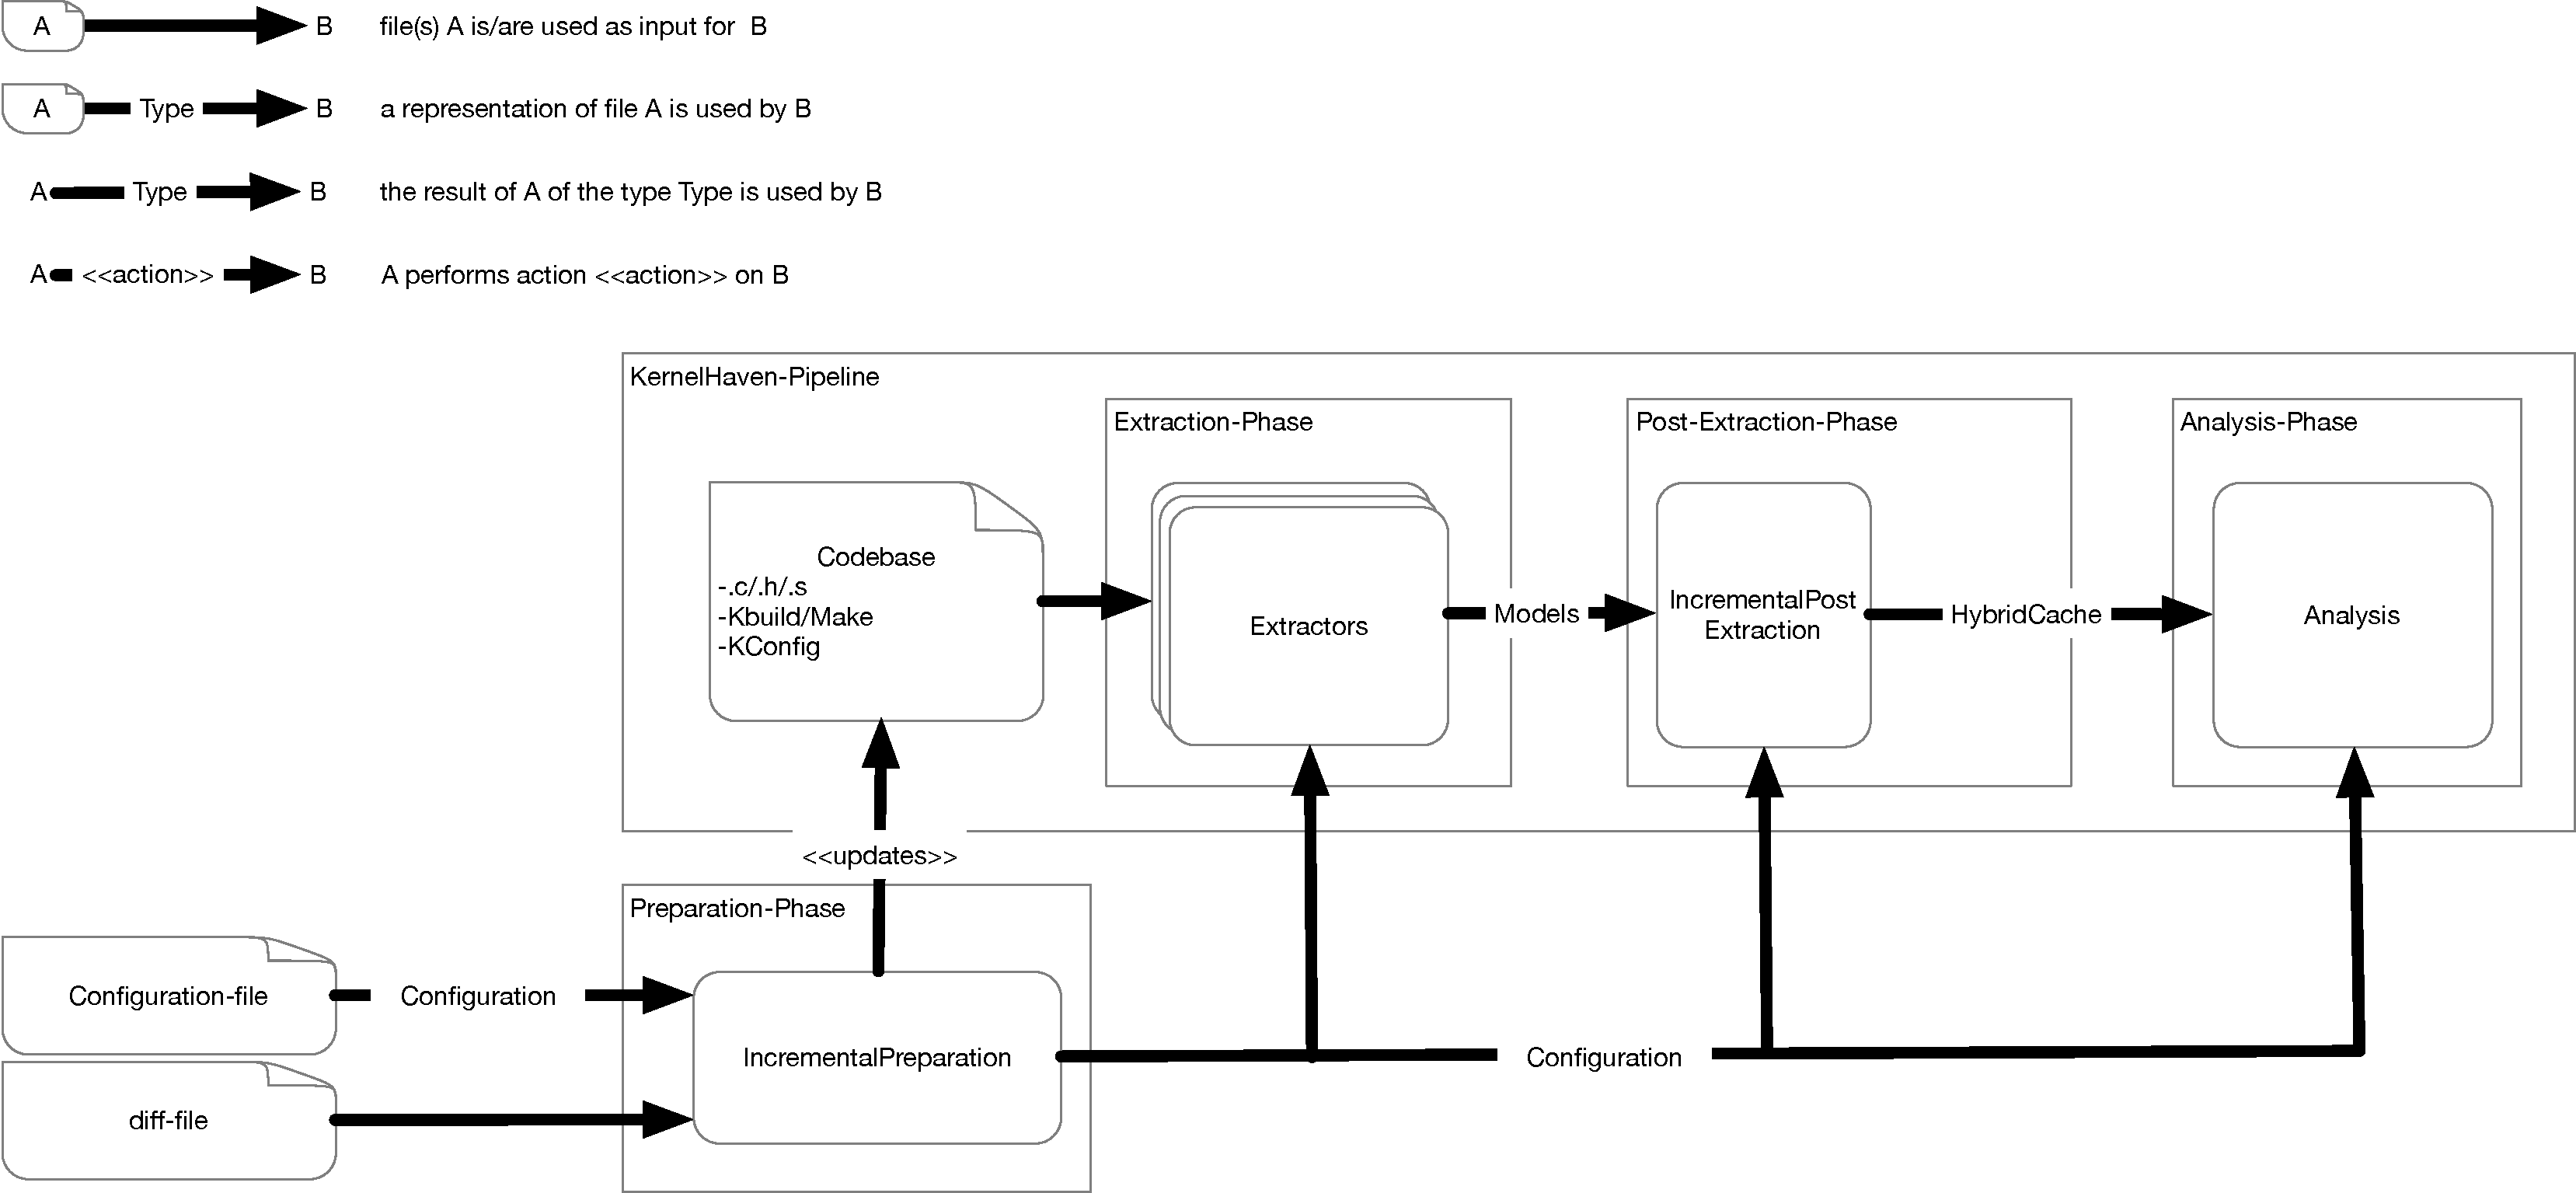
\includegraphics[width=1\textwidth]{img/KernelHavenIncremental.pdf}
  \end{minipage}
\end{figure}



\subsection{Implementation of the Preparation-Phase}\label{preparation-phase}

Because the definition of inputs for the extractors of the Preparation-Component needs to happen before the extraction and analysis itself, it makes sense to run them before an analysis is instantiated. With the \texttt{IPreparation}-interface, KernelHaven offers a mechanism to execute code before the rest of the infrastructure is started. Therefore it allows to modify the configuration that is initially described by a configuration-file. Furthermore other tasks independent of the modifications to the configuration such as applying changes to the codebase may also be executed.

An alternative to this approach would have been to configure extractors from within an analysis-plugin through the implementation of an \texttt{AnalysisComponent} or \texttt{PipelineAnalysis}. In this case the analysis-plugin would have to care about the configuration of extractors and the content of the codebase on the filesystem. This is possible because KernelHaven is implemented as a pull-pipeline. The component at the very end of the pipeline could technically modify the way that prior components work. It would however represent a breach in the data-flow to have the last component modify the inputs and configuration for prior  components. 

In a non-incremental analysis, the definition of the configuration happens before the pipeline is started when writing the configuration-file. Some parameters of the configuration might get overwritten by command line parameters when the pipeline is set up by the \texttt{PipelineConfigurator}, the class responsible for putting all parts together before starting the pipeline - however the configuration is not directly modified from extractors or analyses. Using the \texttt{IPreparation}-interface preserves the data-flow within KernelHaven.

Furthermore, the the \texttt{IPreparation}-interface offers more flexibility to adjust the configuration of KernelHaven as all parts of the infrastructure - even the actual analysis-class itself - can be configured from within an \texttt{IPreparation}-implementation. Therfore the modifiability of the incremental infrastructure is higher than with analysis-classes which may only change the configuration for extractors.

For the incremental infrastructure, the \texttt{IncrementalPreparation}-class implements the \texttt{IPreparation}-interface and merges the changes described by the diff-file with the exisiting codebase. It then continues to filter the files within the codebase to reduce them to a subset that the extraction needs to run on. The configuration then is updated by defining the actual input-files upon which the extractors are run.

The following three sections explain those steps in detail.

\subsubsection{Updating the Codebase}\label{git-apply}

The changes to the codebase are described through a git-diff file. While it is technically possible to create own implementations that apply those changes to files on the filesystem, we use the \texttt{git apply} command. \texttt{git apply} allows to apply changes in git-diff file to a given directory even if that directory is not a git repository. All that is required is command line call from within the folder on which the command should be applied:

\begin{lstlisting}[language=bash]
  $ git apply path/to/git.diff
\end{lstlisting}

 Furthermore \texttt{git apply} also allows to revert changes thereby ensuring the fulfillment of REQ \ref{req:rollback}:
 \begin{lstlisting}[language=bash]
  $ git apply --reverse path/to/git.diff
\end{lstlisting}
 
 A downside to using \texttt{git apply} is that it requires git to be installed on the system that KernelHaven is executed on. However because we assume a git-diff file as input (see REQ \ref{req:git-diff}), it is reasonable to assume that git is most likely already installed on the executing system.

Furthermore there are several advantages to using \texttt{git apply}. As the input is defined by the creation of a git-diff file through the \texttt{git diff} command, also using git to apply the changes ensures compatibility with the file. Therefore we assume that the existing git implementation is less prone to errors than an own implementation or other third party implementations. The integration of \texttt{git apply} results in a low implementation effort as command line calls can easily be realized through javas \texttt{ProcessBuilder}\footnote{ProcessBuilder documentation: \url{https://docs.oracle.com/javase/7/docs/api/java/lang/ProcessBuilder.html}}.

\subsubsection{Filtering of Input Files}\label{filtering-input}

After the codebase was updated, all files represeting variability within the revision that is to be analyzed are available for subsequent processing. To fulfill REQ \ref{req:early-filtering}, a filtering mechanism is implemented. Filters can be configured individually for code-, build-, and variability-files through the configuration-file.

One important resource that the filters use is an abstraction of the git-diff file that was used as input. This abstraction is implemented through the \texttt{DiffFile}-class.
An instance of the \texttt{DiffFile}-object contains an entry for each file that was affected by the changes described in the git-diff file that was used as input. For each entry, one of the following types of change is included:

\begin{itemize}
	\item \texttt{MODIFICATION} \\
	      indicates a modification of the file
	\item \texttt{ADDITION} \\
	      indicates the addition of the file
	\item \texttt{DELETION} \\
	      indicates the deletion of the file 
	\item \texttt{UNDEFINED} \\
	      the type of change should never be undefined. If it is, this indicates that the git-diff file was not properly translated into a \texttt{DiffFile}-object.
\end{itemize}

Furthermore the entries contain information on whether the variability is changed through the according git-diff file. So each entry is assigned one of the following markers aswell:

\begin{itemize}
	\item \texttt{CHANGE} \\
	      indicates changed variability
	\item \texttt{NO\_CHANGE} \\
	      indicates unchanged variability
	\item \texttt{NOT\_A\_VARIABILITY\_FILE}\\
	      indicates that the file was not considered to be a filetype that carries variability information
	\item \texttt{NOT\_ANALYZED}\\
	      indicates that the file was not analyzed at all for variability changes
\end{itemize}

Creating an abstraction of the git-diff file requires that the file itself is read and interpreted. This is done by a \texttt{DiffAnalyzer}, a class that takes the git-diff file used as input and translates it into a \texttt{DiffFile}-object. There are two existing DiffAnalyzers implemented within the incremental infrastructure: the \texttt{SimpleDiffAnalyzer} which only looks for the type of change without considering variability and the \texttt{VariabilityDiffAnalyzer} which also analyses for variability changes. The advantage of the \texttt{SimpleDiffAnalyzer} is that it is faster than the \texttt{VariabilityDiffAnalyzer}. \todo{give numbers here - how much slower? test on initial commit}
Therefore it makes sense to always use the \texttt{SimpleDiffAnalyzer} when variability-information is not needed for filtering. The reason for not handling the interpretation of the git-diff file directly within the filters is that this would result in all three filters having to do the interpretation separately thereby creating computational overhead.

The implementation of the \texttt{VariabilityDiffAnalyzer} relies on previous work which performed a commit based analysis of software product line evolution \cite{ComAn}. The tool used and implemented for this analysis  is called ComAn \cite{ComAn-tool}. Because the paper covers commits to the Linux kernel, the tool is able to process git-diff files describing changes within the codebase of the Linux kernel. 

ComAn allows to extract the number of lines where variability information is modified for each changed file that is described in the git-diff file. This information is used within the \texttt{VariabilityDiffAnalyzer} to determine which files contain variability changes.

The result of the \texttt{DiffAnalyzer} (the DiffFile-object) then gets passed to the filters together with the path to the codebase on the filesystem and a regular expression describing which files to include. Those regular expressions can be configured individually for files related to the code-, build- and variabilitymodel through the configuration file. 

The output of each filter is a list of all the paths that should be included for extraction. Because a separate filter is responsible for each type of model, three lists are created separately for the extractors for build-, variability- and codemodel.
However currently only extractors for the codemodel can handle running on a subset of files within the codebase. As a result, both build- and variabilitymodel need to be extracted from scratch based on the entire codebase as soon as at least one corresponding file with a variability change.

Each of the three separate filters for the code-, build- and variabilitymodel can be configured individually but in some cases one implementation can also be reused for all models. This is because the regular expression may allow sufficient adjustments for each model type. For example a filter that filters for file changes only can process each file in the same exact way no matter what it contains - however by providing a regular expression, it is able to return only files of a certain type. Therefore it is able to filter individually for files of the build-, variability- or codemodel.

 Any filter implementations must extend the abstract \texttt{InputFilter}-class. The following filters are included in the incremental infrastructure - all of which can be applied to code-, build- and variabilitymodel:

\begin{itemize}
\item \texttt{DefaultFilter} \\
    This filter lists all files within the directory of the codebase and filters them using the regular expression on the file-path. If all files representing  the build-, code- or variabilitmodel within the codebase are matched by the regular expression, this filter represents the off option described in REQ \ref{req:optimization}.
\item \texttt{ChangedOnlyFilter} \\
    filters according to the change only option described in REQ \ref{req:optimization}. This filter takes the entries from the \texttt{DiffFile}-object where the file was either marked as Addition or Modification and then filters the file-paths for the regular expression.
\item \texttt{VariabilityChangesFilter} \\
    filters according to the variabilty change only option described in REQ \ref{req:optimization}. This filter filters similar to the \texttt{ChangedOnlyFilter} but only includes the files where the variability was marked as \texttt{CHANGE}. It requires that the git-diff file was analyzed using the \texttt{VariabilityDiffAnalyzer}
\end{itemize}

\subsubsection{Modifying the Configuration}

Based on the results of the filters, the configuration is adjusted. If the list of paths is empty for the code-, variability- or buildmodel, the corresponding extractor does not run as the previous model can simply be reused. To achieve this, the extractors are either turned off or switched on through a configuration option. 

For the codemodel, extractors are able to run on a subset of files within the codebase. Therefore the extractor for the codemodel has a configuration-option to define which files are to be processed. Using this configuration option, the entire list of filtered elements is passed to the codemodel-extractor.

The modifications to the configuration constitute the final step of the Preparation-Phase.

\subsubsection{Implementation of the Post-Extraction-Phase}

In the Post-Extraction-Phase, extraction results are merged with the models extracted in previous iterations and then provided to subsequent analyses. This is implemented in the \texttt{IncrementalPostExtraction}-class. 
\texttt{IncrementalPostExtraction} is written as an analysis plugin because it has a similar point of entry as an analysis: it expects results from the extractors results and processes them. There are two options for implementing an analysis plugin in KernelHaven - one is to implement a single analysis class and the other to implement an analysis-component that can be used in combination with other analysis components to consitute an analysis. Analysis components are implemented by extending the \texttt{AnalysisComponent}-class. A component passes its result on to the next component which then works based on that input. The advantage of the using \texttt{AnalysisComponent} implementation is the possibility for reuse of software components. If multiple different analyses require the same step to be performed somewhere along the way, you can simply reuse the \texttt{AnalysisComponent} that performs that step. For simple pipelines, analysis components may also be combined through the configuration-file. To accomplish this, KernelHaven uses a domain specific language to describe such pipelines. However you can alternatively combine \texttt{AnalysisComponent}s through java code to a \texttt{PipelineAnalysis} if the domain specific language turns out to be insufficient for your use case. In the context of this work, this has been done for the dead code analysis and will be described later (in section \ref{incremental-dead-code-analysis}).

For \texttt{AnalysisComponent}s KernelHaven assumes that those components are chained together and executed strictly one after each other. Not using \texttt{AnalysisComponent}s therefore might hold advantages when his strict pattern needs to be broken - for example by skipping steps or repeating a certain step depending on the result of a subsequent step.

However as the tasks of the Post-Extrection-Phase are mandatory before the Analysis-Phase starts. Therfore reuse of the component that implements the tasks is paramount. Therefore \texttt{IncrementalPostExtraction} is written as an \texttt{AnalysisComponent}.

\subsubsection{Pulling Extractor Results}

\texttt{IncrementalPostExtraction} can pull results from all three extractors in order to merge them with previously extracted models. \texttt{IncrementalPreparation} defines whether new results for code-, build- and variablitymodel need to be extracted by modifying the configuration-object. Using the configuration-object, \texttt{IncrementalPostExtraction} is able to selectively request the result of the code-, build or variabilitymodel-extractor. Therefore only the extractors where the model or parts of the model\footnote{for the codemodel} need to be extracted are started. It is important that the extractors only run when their results are used to prevent computational overhead.

However because of how KernelHaven handles the extraction of models, this required adjustments to the KernelHaven infrastructure. In KernelHaven, an analysis defines which models are needed through its constructor. KernelHaven assumes that it needs to provide all models required by the analysis to it through its extractors. Therefore KernelHaven starts the extractors even before the results of the extractors are requested from within the analysis. 

\texttt{IncrementalPostExtraction} which is implemented as an analysis-plugin potentially requires results from all extractors but may end up requesting none of them. So while its constructor defines all three models as required this does not necessarily match the need to extract them. To overcome this obstacle, a configuration option was implemented in KernelHaven so that the extractor start is delayed until the result of the extractor is requested. While this configuration option may also be used from within the configuration-file for other analyses, it gets set automatically within \texttt{IncrementalPreparation} as soon as not all three models need to be extracted.

An alternative to this approach would have been to provide multiple implementations for the Post-Extraction-Phase. As the extractors are started depending on the models defined in the constructor of the analysis, implementations similar to \texttt{IncrementalPostExtraction} covering each combination of code-, build- and variabilitymodel would have been required. This would have resulted in additional clutter from the classes themselves. Furthermore the PreparationPhase would always need to reconfigure the configuration so that the Post-Extraction-Implementation in use matches the models that need to be extracted. While this has the advantage that no changes to the main KernelHaven infrastructure would be neccessary, this option was disregarded in order to keep the implementaition clutter-free and concise.

KernelHaven does not have configuration-options to directly block the extractors from running. However implementing such options was an option that is technically feasible as it solves the problem for \texttt{IncrementalPostExtraction}. While starting the extractors before the analysis requests results can be seen as an optimisation option, blocking extractor execution completely even if an analysis requires the model does contradict the design of KernelHaven where the analysis dictates which models it needs.

\subsubsection{Merging Extractor Results}

Having access to the results of the current execution of the extractors is not enough as an analysis may need the complete models and only a subset of them might have been newly extracted. Therefore extracted models get stored for access in subsequent iterations of an incremental analysis. The very first execution of the incremental infrastructure always has do do a full extraction while subsequent executions perform updates on the initially extracted models. However it is not sufficient to simply update the model - the previous version of the model must be accessible in order to allow a rollback as described in REQ \ref{req:rollback}. The storage of the current and previous version of the models is implemented in the \texttt{HybridCache}.

\texttt{HybridCache} itself uses the same caching-implementation that KernelHaven uses for its cache. This means that it works based on the filesystem and writes serialized models to a cache-folder. The variability- and build-model are represented by a single file while the codemodel is represented by multiple files - meaning that each sourcefile constituting the codemodel is represented by one file within \texttt{HybridCache}.
 
 In contrast to KernelHavens cache however, the \texttt{HybridCache} uses multiple folders to store its files. The core idea is to have one folder describing all current models called 'current' and another folder called 'history' describing the changes that were applied to the previous models in comparison. Effectively the 'history'-folder repesents a change history of the models but only stores the version of each model-file before the most recent change made to it. 
 If a model-file is replaced by a newer version, the replaced file is copied to the 'history'-folder. The same holds true for model-files that are deleted. In both of those instances, the files are copied to a folder called 'replaced' within the hybrid-cache directory. The reason for moving deleted files to the same folder as replaced files is that they can be handled in the same way when a rollback is triggered. Both the deleted and replaced files can be copied back to the current folder thereby reverting the changes made.
 
To determine which files were deleted, \texttt{IncrementalPostExtraction} again uses a \texttt{DiffFile}-object. Because the git-diff file has to be interpreted to obtain a \texttt{DiffFile}-object within \texttt{IncrementalPreparation} aswell, the \texttt{DiffFile}-object can be loaded from a serialized version that got created through \texttt{IncrementalPreparation} earlier. While loading an the \texttt{DiffFile} from the harddrive is not as desirable as passing the object directly from \texttt{IncrementalPreparation} to \texttt{IncrementalPostExtraction}, KernelHaven does not allow objects to be passed between an \texttt{IPreparation} and Analysis-Plugins. If no serialized version of the \texttt{DiffFile}-object created in the \texttt{IncrementalPreparation} can be found, \texttt{IncrementalPostExtraction} uses \texttt{SimpleDiffAnalyzer} to interpret the git-diff file. An alternative to storing a serialized version of the \texttt{DiffFile} within the filesystem would have been to insert it into the configuration-object. While technically feasible, this would result in a misuse of the configuration-object as its purpose is to transport configuration options, not to store java-objects within KernelHaven. Another option would have been to always newly interpret the git-diff file. \texttt{SimpleDiffAnalyzer} is able to handle the interpretation of a git-diff file quickly enough so that it does not have a noteworthy impact on the overall performance of an incremental analysis. However loading an already interpreted version is still faster. Furthermore storing a serialized version of the git-diff file allows the user to inspect how the changes introduced through the git-diff file were interpreted. Thereby he is provided with further insight on the changes introduced beyond the analysis results.
 
 On top of deleting and replacing files it is also possible that new model-files get added to the current model-files. If a file is added, an empty file carrying the same name as the added file is created within a subfolder of the 'history'-folder - the 'added'-folder. When a rollback is triggered all files in the current directory where a file with the same name exists in the 'added'-folder get deleted.
 
After an incremental analysis terminates, the history-folder stays intact so that a rollback can be triggered. 
However when starting a subsequent run of the incremental analysis, the contents of the 'history'-folder can be wiped as the history is no longer needed. Instead a new history has to be build for the current execution. Wiping the 'history'-folder equates to setting the content of the 'current'-folder as reference for future 'history'-entries. This allows a new history to be built for another execution of the incremental analysis.
  
 \texttt{HybridCache} does not actually compare the contents of a file with the previous version when a model is to be written to the cache. So when a newly extracted model is actually the same as the model represented in the present mode-file, the newly extracted model is still handled as a replacement for it. 
  
 By always storing both model-files, a comparison between those version becomes possible. At the same time, we can still determine all extraction results of the current iteration through the \texttt{HybridCache}. This is because an extracted file will always have a counterpart within the history-folder.
   
 A benefit of the \texttt{HybridCache} implementation is that it does not require as much storage space as versioning systems such as git or svn as only the two most current revisions need to be stored. It also does not require costly diffs between revisions to operate. Furthermore \texttt{IncrementalPostExtraction} remains independent of external libaries or tools \footnote{The incremental infrastructure itself does rely on git for applying changes to the codebase as mentioned in \autoref{preparation-phase}. The incremental infrastructure therefore is not completely independent from other tools.}.
 
As \texttt{HybridCache} does allow access to both the current and previous model, the instance of the \texttt{HybridCache} used within \texttt{IncrementalPostExtraction} is also passed on to the next \texttt{AnalysisComponent}. 
  
\subsection{Implementation of incremental Analyses}

An \texttt{AnalysisComponent} using the \texttt{HybridCache} as input has access to all models in both the previous and current version. In order to make the implementation of an incremental analysis easier, \texttt{HybridCache} also allows to directly obtain the parts of the codemodel that did change. \texttt{AnalysisComponent}s implemented specifically for the incremental infrastructure may therefore work directly with an \texttt{HybridCache}-object as input. 

Non-incremental \texttt{AnalysisComponent}-classes that directly work with code-, build- or variabilitymodel assume different inputs. For those \texttt{AnalysisComponents} the expected inputs are three distinct \texttt{AnalysisComponent}s which provide code, build- and variabilitymodel. Each of those three components are passed to the non-incremental component through the constructor of the class as shown in the following code snippet:

\begin{lstlisting}[language=java]
/* Dead Code Analysis returning Dead Code Blocks as a result */
public class DeadCodeFinder extends AnalysisComponent<DeadCodeBlock> {
    /**
     * Creates a dead code analysis.
     */
    public DeadCodeFinder(Configuration config, 
        AnalysisComponent<VariabilityModel> vmComponent, 
        AnalysisComponent<BuildModel> bmComponent, 
        AnalysisComponent<SourceFile> cmComponent) {
        ...
    }
\end{lstlisting}

In order to comply with the input-definition an adaptation is needed. This adaptation can be achieved through the use of the \texttt{HybridCacheAdapter}. \texttt{HybridCacheAdapter} is able to create three distinct components providing the three models for usage in an \texttt{AnalysisComponent}. As it has to provide three different kinds of results to the next \texttt{AnalysisComponent} it can not use the default interface of \texttt{AnalysisComponent} for passing results. This is because that interface only allows to pass results of one specific kind. Therefore the access to the generated components that provide the model is achieved through get()-methods and not through the default interface. 

\autoref{hybrid-cache} visualizes the usage of \texttt{HybridCacheAdapter} through an example. \texttt{IncrementalPostExtraction} defines its result as an \texttt{HybridCache}-object. \texttt{HybridCacheAdapter} uses that result but does not provide any result through the default interface. Instead it defines an empty output trough the usage of \texttt{Void} as result type. However it provides three \texttt{OutputComponent}s that are accessible through getters. The \texttt{OutputComponent}-class is a private class within the \texttt{HybridCacheAdapter} that is used as a wrapper for the models. Because an \texttt{OutputComponent} does extend the \texttt{AnalysisComponent}-class, it can be used as input for a subsequent \texttt{AnalysisComponent} - in this case the \texttt{DeadCodeAnalysis}. The \texttt{DeadCodeAnalysis} then computes the final result.

\begin{figure}[h] 
  \centering
  \begin{minipage}[b]{1\textwidth} 
    \caption[Usage of the HybridCacheAdapter]{Usage of the HybridCacheAdapter}\label{hybrid-cache}
    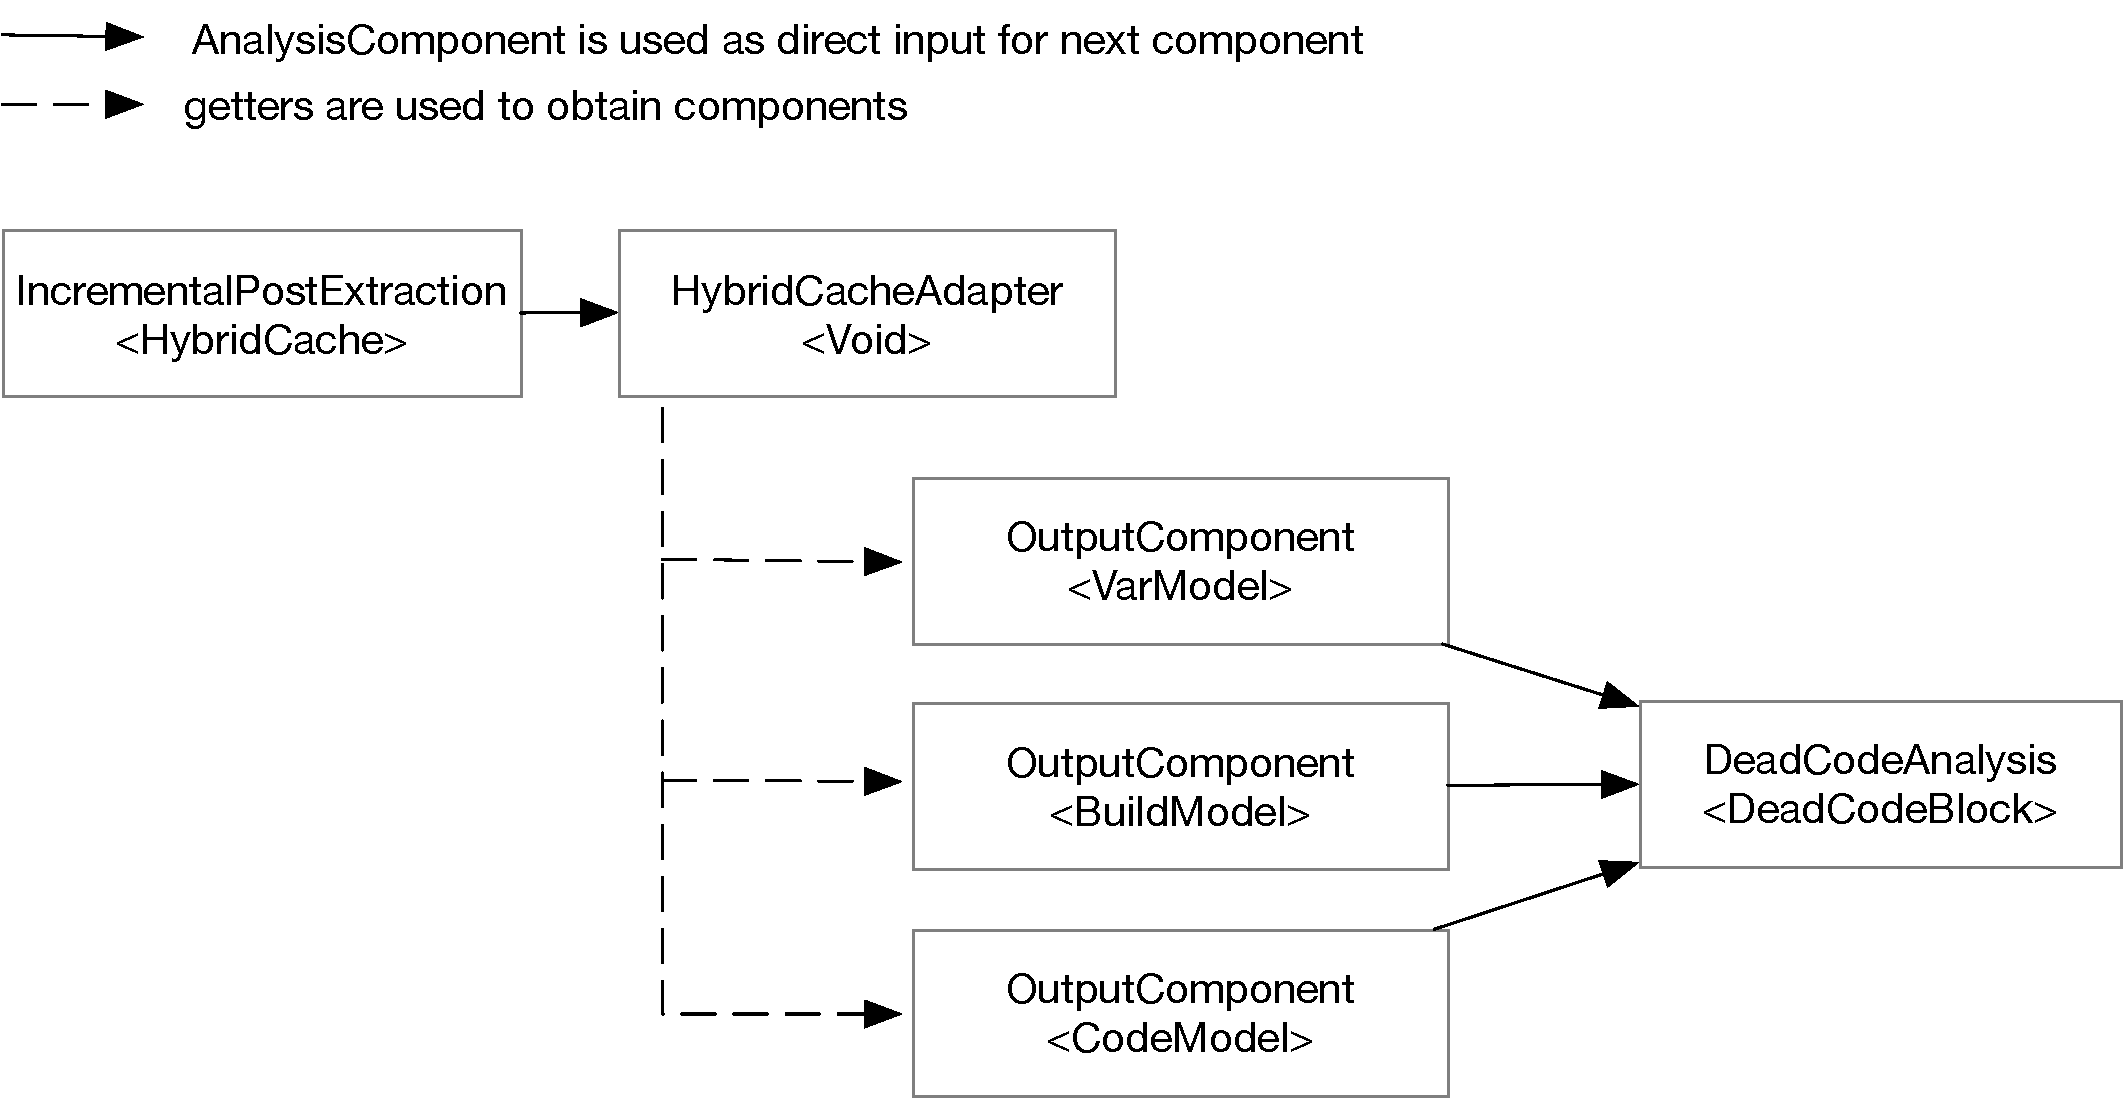
\includegraphics[width=1\textwidth]{img/HybridCacheAdapter.pdf}
  \end{minipage}
\end{figure}

Adapting the input for the analysis is not the only purpose of the \texttt{HybridCacheAdapter} as it also defines which parts of the codemodel are passed on to the \texttt{AnalysisComponent}. Some  \texttt{AnalysisComponent}s like the \texttt{FeatureEffectAnalysis} might always need the complete codemodel and are therefore able to profit from faster extraction times through the incremental infrastructure. In fact existing non-incremental analysis is able to process complete models as this is what the KernelHaven infrastructure provides by default. It is therefore worth noting that the easiest way to adapt an analysis  is to pass the entire model to it through the \texttt{HybridCacheAdapter}.

However the \texttt{DeadCodeAnalysis} may only need to access the part of the model that was modified as processing unchanged parts of the model does not always induce new results. Therefore the \texttt{HybridCacheAdapter} can either be used to return a complete codemodel or just the changed parts. The implementation of an incremental version of the \texttt{DeadCodeAnalysis} itself is explained in the next section.

As the \texttt{HybridCacheAdapter} is meant for quick adaptation of existing analyses, it only provides generic functionality for filtering the codemodel by allowing to only provide the changed parts of the model. If filters are specifically designed to work for one analysis, they should be implemented within that analysis itself utilizing the full capabilities of \texttt{HybridCache} instead of relying on an adapter. This is why in contrast to \texttt{IncrementalPreparation} where custom implementations for \texttt{InputFilter}s are allowed for filtering files within the codebase, the \texttt{HybridCache} does not provide such an interface for filtering the codemodel.

\subsubsection{Incremental Dead Code Analysis} \label{incremental-dead-code-analysis}

The \texttt{DeadCodeFinder} is an \texttt{AnalysisComponent} implemented in the \texttt{UndeadAnalyzer}-plugin of KernelHaven. It uses the code-, build- and variabilitymodel to compute results. The codemodel is represented by a collection of \texttt{SourceFile}-objects each representing the model of a single sourcefile from the codebase.

The analysis iterates over all \texttt{SourceFile}-objects and separately checks them for dead code blocks. The constraints defined through the build- and variabilitymodel are included for the identification of such code blocks. Because every model represented by a \texttt{SourceFile} is considered separately, changes in other parts of the codemodel do not impact the result of an unchanged parts. Therefore unchanged parts of the model do not need to be analyzed again if only the codemodel changed. It is sufficient to only analyze the parts of the codemodel that did change.

If however the variability- or the buildmodel did change, the restrictions that were used to analyze the each part of the codemodel have changed aswell. As a result, the entire codemodel has to be processed again within the analysis.

Therefore for implementing an incremental version of the \texttt{DeadCodeAnalysis} we have to consider the following two possibilities:

\begin{enumerate}
 \item variability- and buildmodel did not change
 \begin{itemize}
 	\item only provide new parts of the codemodel to \texttt{DeadCodeFinder}
 \end{itemize}
  \item variability- or buildmodel did change
 \begin{itemize}
 	\item provide complete codemodel to \texttt{DeadCodeFinder} (including parts of the model that were extracted in previous executions of the incremental analysis)
 \end{itemize}
\end{enumerate}

The current variability- and buildmodel are always provided to the \texttt{DeadCodeFinder} as they are required to process each \texttt{SourceFile}-object. The following code shows the main part of the incremental implementation for the Dead Code Analysis\footnote{for the complete implementation refer to \url{https://github.com/KernelHaven/IncrementalDeadCodeAnalysis}}:

\begin{lstlisting}[language=java]
// Determine whether only a part of the codemodel must be analyzed
boolean partialAnalysis = !updatedBuildModel && !updatedVariabilityModel;

// Create the adapter
HybridCacheAdapter hca = new HybridCacheAdapter(config,
    new IncrementalPostExtraction(config, 
        getCmComponent(), 
        getBmComponent(), 
        getVmComponent()
    ),
    partialAnalysis);

// Create the AnalysisComponent performing the Dead Code Analysis
DeadCodeFinder dcf = new DeadCodeFinder(config, 
    hca.getVmComponent(), 
    hca.getBmComponent(),
    hca.getCmComponent());

return dcf;
\end{lstlisting}

\newpage
\section{Evaluation}

The evaluation of the incremental infrastructure will be performed to shed light on the performance gain as well as constistency of the results with those of a non-incremental analysis. The incremental infrastructure with the Dead Code Analysis will be compared against the non-incremental Dead Code Analysis implemented for KernelHaven. Both systems will mostly be using the same configuration for running with the exception being the additional parameters required for incremental analyses and of course the analysis-class itself.

After computing some first preliminary results using both the incremental infrastructure and a non-incremental analysis in KernelHaven it became clear that the evaluation could not be performed for a large set of commits in a timely manner without further changes. This is because the non-incremental analysis always has to perform SAT-solving for all of the conditions imposed by the models for each commit. With the hardware at hand, about three iterations of the analysis could be performed per day. However the existing Dead Code Analysis was not multithreaded. In order to accomplish a higher number of analyzed commits, we chose to create a multithreaded version of the Dead Code Analysis. In doing so, we were able to achieve appoximately 35 analyses per day on our reference system.

Those changes enabled the timely availabily of reference results for the incremental analysis to compare against. In order to keep the results compareable, the incremental version of the enalayis was also adjusted to support multithreaded operation. Those changes however do reduce the meaningfulness of comparisons against other tools that do not run multithreaded such as Undertaker \cite{Tartler:2011:FCC:1966445.1966451}. Undertaker is a tool that was developed prior to KernelHaven, supports the extraction of code models and is able to perform Dead Code Analysis on them. Given that Kernelhaven has an extractor plugin that leverages the extraction functionality of Undertaker, a comparison against the original Undertaker-tool would certainly have been interesting.

The data used for evaluation consists of 307 commits to the main branch of the Linux kernel source tree \cite{linux}. Each commit was transformed into a git-diff file that then was directly used as input for the incremental analysis. The non-incremental reference results were also computed based on the diff-files. However the changes described through each git-diff file were applied to the codebase before the execution of KernelHaven itself as the non-incremental Dead Code Analysis expects a codebase that it can work with directly. The table below shows the exact range of commits used and how they were represented for the evaluation.

\begin{tabular}{l | l | l}
	Commit-Hash & Description & File \\ \hline
	4fbd8d194f06c8a3fd2af1ce560ddb31f7ec8323 & Linux 4.15-rc1 & 00001-git.diff \\
	... & ... & ... \\
	d8a5b80568a9cb66810e75b182018e9edb68e8ff & Linux 4.15  & 00307-git.diff \\
\end{tabular}

To automate the generation of results, a collection of bash-scripts\footnote{\url{https://github.com/moritzfl/IncrementalAnalysesEvaluation}} was created. The github-project containing the bash-scripts also includes the git-diff files used for evaluation. The results computed by KernelHaven are attached to a release within the github-project. The reference system used for execution a virtual linux machine hosted on VMware ESXi \cite{ESXi-f0l} with 24 configured CPU-cores and 64GB RAM while the host system itself had access to 12 phyisical and 24 logical CPU cores clocked at 2.20 GHz each.

\subsection{Early Evaluation results}

The evaluation uses the results of a non-incremental dead code analysis as reference.  The reference was compared against two incremental analyses configured according to the variability-change-only and a change-only options described in REQ \ref{req:mandatory-filters}.

When running the evaluation for the first time, some issues were identified that needed to be fixed. Therefore the results of the incrmental executions were not entirely consistent with the reference. However they were close enough to assume that resolving those issues would produce consistent results.

The first issue that was noticed was that the execution of the bash-script for the reference-system was stopped unexpectedly. The interruption occured when applying the changes described by the file 00129-git.diff to the codebase. This is because this file is empty as the commit it represents was a merge-commit to the main branch of the Linux kernel that did not actually change anything. Therefore the commit was skipped for all subsequent evaluation executions.

Looking at the isolated results of the reference, it became clear that the reference had issues analyzing some states of the codebase. A total of 71 reference analysis executions resulted in no dead code blocks while all preceding and subsequent analysis results contained such blocks. Investigating the log-files we found that the issue was most likely due to the \texttt{KConfigReaderExtractor} not being able to extract the model from the codebase. Upon further investigation and using the original KConfigReader-tool, the assumed cause was confirmed\todo{insert reference to issue on github}. However it revealed a related bug for the incremental execution as those did still find dead code blocks. This is because when the extraction of variability-and buildmodel failed, the incremental infrastructure provided the previous models to the analysis. It was implemented in a way that it only replaced old models with new one. This has now been fixed as a failed execution of the buildmodel or variabilitymodel now results in the deletion of the model from the HybridCache\footnote{rollback is still possible}.

Additionally, a bug within the VariabilityChangeFilter was found that resulted in files not being marked as \texttt{VariabilityChange.CHANGE} in cases where ComAn could not extract variability information. While this is only relevant for a small number of cases, this behaviour represents an important fallback mechansism. While a false positive might require additional processing, assuming changed variability in such cases ensures that the extracted models represent the codebase correctly.

However there were also expected deviations within the results of the variabilty-only-filter execution compared to the reference. Using the \texttt{VariabilityChangeFilter}, the code-model for a single codefile only gets rebuilt when variability-information within that file is modified. When a change is made within a codefile that does not change variability-information, it might still change the position of dead code blocks. A trivial example would be an inserted comment line right before an \texttt{\#ifdef}-block. This moves the block down by one line. However the codemodel does not get extracted again. The codemodel still contains the information that \texttt{\#ifdef}-blocks exist within the same codefile but only has access to the previous linenumber. As a result, when an analysis is performed on the entire codemodel after an update to the build- or variabilitymodel, the linenumbers do not match the result of the reference.

Another deviation from the reference result stems from the fact that only variabilty-changes are considered to be relevant. In the reference execution, a dead code analysis was performed covering every single sourcefile in the codebase. This is not the case for the variability-change-only execution as it only covers the files where variability-information was modified.

The following entry was present in the reference result for \texttt{00001-git.diff} but not for the incremental result using the \texttt{VariabilityChangeFilter}:

\begin{lstlisting}
drivers/net/arcnet/com90xx.c;(CONFIG_ARCNET_COM90xx || CONFIG_ARCNET_COM90xx_MODULE) && (CONFIG_ARCNET || CONFIG_ARCNET_MODULE);606;610;0
\end{lstlisting}

Looking at \texttt{drivers/net/arcnet/com90xx.c} we can see that the dead code block actually got inserted on purpose and does not represent a modification to variability:

\begin{lstlisting}
#if 0
    /* don't do this until we verify that it doesn't hurt older cards! */
    arcnet_outb(arcnet_inb(ioaddr, COM9026_REG_RW_CONFIG) | ENABLE16flag, ioaddr, COM9026_REG_RW_CONFIG);
#endif
\end{lstlisting}

The reference results therefore contained more dead code blocks as they also included those from files where the variability was not changed. 

However when ignoring additional entries for non-variablity-related dead code blocks within the reference results, the variability-change-only results matched the reference results. Relevant entries that are related to variability can be identified because their presence condition has to contain the \texttt{CONFIG\_} prefix. In the result the presence condition is denoted as the element behind the last semicolon. In our example the presence condition is \texttt{0}. It does not contain \texttt{CONFIG\_} and therefore is not related to variability.

Considering the results, the variability-change-only option is suitable when dead code blocks related to variabilty are the major concern. If however all dead-code-blocks should be found, one should be able to use the \texttt{ChangeFilter} for the codemodel instead. That way, all changes within the codemodel get analyzed while changes to build- and variabilitymodel are still processed using the \texttt{VariabilityChangeFilter}. This configuration seems practical, because the extraction and analysis of single codefiles does only require a small computational effort. However updates to the build- or variabilitymodel would result in costly computations as they require a full analysis covering the entire codemodel.

\subsection{Non-Incremental: Results}

\subsection{Incremental: ChangeFilter Results}

\subsection{Incremental: VariabilityChangeFilter Results}

\subsection{Incremental: No Filter}


%\Bibliography
\newpage

\bibliography{sources}


\end{document} 